\documentclass[10pt,a4paper]{article}
\usepackage[UTF8,fontset = windows]{ctex}
\setCJKmainfont[BoldFont=黑体,ItalicFont=楷体]{华文中宋}
\usepackage{amssymb,amsmath,amsfonts,amsthm,mathrsfs,dsfont,graphicx}
\usepackage{ifthen,indentfirst,enumerate,color,titletoc}
\usepackage{tikz}
\usepackage{makecell}
\usepackage{longtable}
%\usepackage{mathptmx}

\usetikzlibrary{arrows,calc,intersections,patterns,decorations.pathreplacing,angles}
\usepackage[bf,small,indentafter,pagestyles]{titlesec}
\usepackage[top=1in, bottom=1in,left=0.8in,right=0.8in]{geometry}
\renewcommand{\baselinestretch}{1.65}
\newtheorem{defi}{定义~}
\newtheorem{eg}{例~}
\newtheorem{ex}{~}
\newtheorem{rem}{注~}
\newtheorem{thm}{定理~}
\newtheorem{coro}{推论~}
\newtheorem{axiom}{公理~}
\newtheorem{prop}{性质~}
\newcommand{\blank}[1]{\underline{\hbox to #1pt{}}}
\newcommand{\bracket}[1]{(\hbox to #1pt{})}
\newcommand{\onech}[4]{\par\begin{tabular}{p{.9\textwidth}}
A.~#1\\
B.~#2\\
C.~#3\\
D.~#4
\end{tabular}}
\newcommand{\twoch}[4]{\par\begin{tabular}{p{.46\textwidth}p{.46\textwidth}}
A.~#1& B.~#2\\
C.~#3& D.~#4
\end{tabular}}
\newcommand{\vartwoch}[4]{\par\begin{tabular}{p{.46\textwidth}p{.46\textwidth}}
(1)~#1& (2)~#2\\
(3)~#3& (4)~#4
\end{tabular}}
\newcommand{\fourch}[4]{\par\begin{tabular}{p{.23\textwidth}p{.23\textwidth}p{.23\textwidth}p{.23\textwidth}}
A.~#1 &B.~#2& C.~#3& D.~#4
\end{tabular}}
\newcommand{\varfourch}[4]{\par\begin{tabular}{p{.23\textwidth}p{.23\textwidth}p{.23\textwidth}p{.23\textwidth}}
(1)~#1 &(2)~#2& (3)~#3& (4)~#4
\end{tabular}}
\begin{document}
\begin{enumerate}[1.]


\item 已知数列$\{a_n\}$满足$a_n=pn+q$($p,q$为常数, $n\in \mathbf{N}^*$), 求证: $\{a_n\}$是等差数列.\\
解答在这里  因为$a_{n+1}-a_n=[p(n+1)+q]-(pn+q)=p$($n\in \mathbf{N}^*$), 所以$\{a_n\}$是等差数列, 显然, 常数$p$是它的公差.
\item 已知数列前$n$项和$S_n=An^2+Bn+C$, 试证明此数列从第二项起, 构成一个等差数列.\\
解答在这里  由已知, $a_n=S_n-S_{n-1}=An^2+Bn+C-[A(n-1)^2+B(n-1)+C] =A(2n-1)+B=2An+(B-A)$($n\ge 2$, $n\in \mathbf{N}^*$). 于是$a_{n+1}-a_n=[2A(n+1)+(B-A)]-[2An+(B-A)]=2A$($n\ge 2$, $n\in \mathbf{N}^*$), 故$\{a_n\}$从第二项起, 构成一个等差数列.
\item 已知数列$\{a_n\}$满足$a_1=1$, $S_n=\dfrac{(n+1)a_n}2$($n\in \mathbf{N}^*$), 求通项$a_n$的表达式.\\
解答在这里 由已知, 得$2S_n=(n+1)a_n$($n\in \mathbf{N}^*$), $2S_{n-1}=na_{n-1}$($n\ge 2$, $n\in \mathbf{N}^*$),
两式相减, 得$2a_n=(n+1)a_n-na_{n-1}$, 即$(n-1)a_n=na_{n-1}$,
所以$\dfrac{a_n}{{a_{n-1}}}=\dfrac n{n-1}$($n\ge 2$, $n\in \mathbf{N}^*$),
于是有$\dfrac{a_2}{a_1}=\dfrac 21,\dfrac{a_3}{a_2}=\dfrac 32,\dfrac{a_4}{a_3}=\dfrac 43,\cdots,\dfrac{a_n}{a_{n-1}}=\dfrac n{n-1}$($n\ge 2$, $n\in \mathbf{N}^*$).
以上诸式相乘, 得$a_n=na_1=n$($n\ge 2$, $n\in \mathbf{N}^*$).又$a_1=1$, 所以$a_n=n$($n\in \mathbf{N}^*$).
\item 在等差数列$\{a_n\}$中, 已知$a_2+a_7+a_8+a_{13}=6$, 求$a_6+a_9$.\\
解答在这里 因为$a_2+a_{13}=a_7+a_8=a_6+a_9$, 所以$a_6+a_9=3$.
\item 在等差数列$\{a_n\}$中, 已知$S_{11}=66$, 求$a_6$.
解答在这里 因为$S_{11}=\dfrac{11(a_1+a_{11})}2=\dfrac{11\times 2a_6}2=11a_6=66$, 所以$a_6=6$.
\item 项数为奇数的等差数列$\{a_n\}$中, 已知奇数项之和为$12$, 偶数项之和为$10$, 求它的项数和中间项.\\
解答在这里  设有$2n-1$项, 则由题意, 得
$\dfrac{S_\text{奇}}{S_\text{偶}}\text=\dfrac{\dfrac{({a_1}+{a_{2n-1}})n}2}{\dfrac{({a_2}+{a_{2n-2}})(n-1)}2}=\dfrac n{n-1}=\dfrac{12}{10}=\dfrac 65$, 所以$n=6$, 故此数列共有$11$项.
又$S_\text{奇}-S_\text{偶}=(a_1+a_3+a_5+\cdots +a_{11})-(a_2+a_4+a_6+\cdots +a_{10})=a_1+(a_3-a_2)+(a_5-a_4)+\cdots +(a_{11}-a_{10})=a_1+5d=a_6=12-10=2$, 所以中间项$a_6=2$.
\item 在等比数列$\{a_n\}$中, 已知前$10$项和为$5$, 前$20$项和为$15$, 求前$30$项和.\\
解答在这里  记$A=a_1+a_2+\cdots +a_{10}$, $B=a_{11}+a_{12}+\cdots +a_{20}$, $C=a_{21}+a_{22}+\cdots +a_{30}$, 则$A=5$, $B=S_{20}-S_{10}=10$.
因为$A,B,C$成等比, 所以$C=\dfrac{B^2}A=\dfrac{100}5=20$, 故$S_{30}=A+B+C=35$.
\item 求数列$1,1+a,1+a+a^2,1+a+a^2+a^3,\cdots,1+a+a^2+\cdots +a^{n-1}, \cdots$的前$n$项和$S_n$.\\
解答在这里  (1) 若$a=1$, 则$a_n=n$, 于是$S_n=1+2+3+\cdots +n=\dfrac{n(n+1)}2$.\\
(2) 若$a\ne 1$, 则$a_n=\dfrac{1-{a^n}}{1-a}$, 于是
$S_n=\dfrac{1-a}{1-a}+\dfrac{1-{a^2}}{1-a}+\dfrac{1-{a^2}}{1-a}+\cdots +\dfrac{1-{a^n}}{1-a}=\dfrac 1{1-a}[n-(a+a^2+a^3+\cdots +a^n)]=\dfrac 1{1-a}[n-\dfrac{a(1-{a^n})}{1-a}]$.
\item 求和: $1+\dfrac 1{1+2}+\dfrac 1{1+2+3}+\cdots +\dfrac 1{1+2+\cdots +n}$($n\in \mathbf{N}^*$).\\
解答在这里  因为$a_k=\dfrac 1{1+2+\cdots +k}=\dfrac 2{k(k+1)}$.
所以$S_n=2[\dfrac 1{1\times 2}+\dfrac 1{2\times 3}+\cdots +\dfrac 1{n(n+1)}]=2[(1-\dfrac 12)+(\dfrac 12-\dfrac 13)+\cdots +(\dfrac 1n-\dfrac 1{n+1})]=2(1-\dfrac 1{n+1})=\dfrac{2n}{n+1}$.
\item 求和: $a+2a^2+3a^3+\cdots +na^n$($n\in \mathbf{N}^*$).\\
解答在这里  记$S_n=a+2a^2+3a^3+\cdots +(n-1)a^{n-1}+na^{n+1}$,
则$aS_n=2a^2+3a^3+\cdots +(n-2)a^{n-1}+(n-1)a^n+na^{n+1}$, 两式相减, 得
$(1-a)S_n=(a+2a^2+3a^3+\cdots +a^n)-na^{n+1}$.
若$a=1$, 则$S_n=1+2+\cdots +n=\dfrac{n(n+1)}2$; 若$a\ne 1$, 则$S_n=\dfrac{a(1-{a^n})}{{{(1-a)}^2}}-\dfrac{n{a^{n+1}}}{1-a}$.
\item 已知数列$6, 9, 14, 21, 30, \cdots$, 其中相邻两项之差成等差数列, 求它的通项.\\
解答在这里  因为$a_2-a_1=3$, $a_3-a_2=5$, $a_4-a_3=7$, $\cdots$, $a_n-a_{n-1}=2n-1$, 各项相加得$a_n-a_1=3+5+7+\cdots +(2n+1)$,
所以$a_n=6+3+5+7+\cdots +(2n+1)=n^2+5$($n\in \mathbf{N}^*$).
\item 若$1\times 2^2+2\times 3^2+3\times 4^2+\cdots +n(n+1)^2=\dfrac{n(n+1)}{12}(an^2+bn+c)$对$n\in \mathbf{N}^*$恒成立, 求$a,b,c$的值.\\
解答在这里  左边$=\sum\limits_{k=1}^nk(k+1)^2=\sum\limits_{k=1}^nk^3+2\sum\limits_{k=1}^nk^2+\sum\limits_{k=1}^nk=\dfrac{n^2(n+1)^2}4+\dfrac{n(n+1)(2n+1)}3+\dfrac{n(n+1)}2$
$=\dfrac{n(n+1)}{12}[3n(n+1)+4(2n+1)+6]=\dfrac{n(n+1)}{12}(3n^2+11n+10)$, 所以$a=3,b=11,c=10$.
\item 若数列$\{a_n\}$满足$a_1=2$, $a_{n+1}-a_n+1=0$($n\in \mathbf{N}^*$), 则此数列的通项$a_n$等于\bracket{20}.
\fourch{$n^2+1$}{$n+1$}{$1-n$}{$3-n$}
\item 若数列$\{a_n\}$的通项公式是$a_n=2(n+1)+3$, 则此数列\bracket{20}.
\twoch{是公差为$2$的等差数列}{是公差为$3$的等差数列}{是公差为$5$的等差数列}{不是等差数列}
\item 若$m,a_1,a_2,n$和$m,b_1,b_2,n$($m\ne n$)分别是两个等差数列, 则$\dfrac{{a_2}-{a_1}}{{b_2}-{b_1}}$的值为\bracket{20}.
\fourch{$\dfrac 23$}{$\dfrac 34$}{$\dfrac 32$}{$\dfrac 43$}
\item 若等差数列$\{a_n\}$的前三项依次为$a-1,a+1,2a+3$, 则此数列的通项$a_n$等于\bracket{20}.
\fourch{$2n-5$}{$2n-3$}{$2n-1$}{$2n+1$}
\item 在等差数列$\{a_n\}$中, 若$a_3+a_4+a_5+a_6+a_7=450$, 则$a_2+a_8$等于\bracket{20}.
\fourch{$45$}{$75$}{$180$}{$320$}
\item 在等差数列$\{a_n\}$中, 已知$a_1+a_4+a_7=39$, $a_2+a_5+a_8=33$, 则$a_3+a_6+a_9$的值是\bracket{20}.
\fourch{$30$}{$27$}{$24$}{$21$}
\item 在递增的等差数列$\{a_n\}$中, 已知$a_3+a_6+a_9=12$, $a_3a_6a_9=28$, 则通项$a_n$等于\bracket{20}.
\fourch{$n-2$}{$16-n$}{$n-2$或$16-n$}{$2-n$}
\item 若等差数列$\{a_n\}$的公差$d$不为零, 且$a_1\ne d$, 前$20$项之和$S_{20}=10M$, 则$M$等于\bracket{20}.
\fourch{$a_6+a_5$}{$a_2+2a_{10}$}{$2a_{10}+d$}{$10a_2+d$}
\item 在等差数列$\{a_n\}$中, 已知前$4$项和是$1$, 前$8$项和是$4$, 则$a_{17}+a_{18}+a_{19}+a_{20}$的值等于\bracket{20}.
\fourch{$7$}{$8$}{$9$}{$10$}
\item 在等差数列$\{a_n\}$中, 若前$15$项的和$S_{15}=90$, 则$a_8$等于\bracket{20}.
\fourch{$6$}{$\dfrac{45}4$}{$12$}{$\dfrac{45}2$}
\item 若数列$\{a_n\}$满足$a_{n+1}=\dfrac{3a_n+2}3$, 且$a_1=0$, 则$a_7=$\blank{50}.
\item 若等差数列$\{a_n\}$满足$a_7=p$, $a_{14}=q$($p\ne q$), 则$a_{21}=$\blank{50}.
\item 首项为$-24$的等差数列从第$10$项开始为正数, 则公差$d$的取值范围是\blank{50}.
\item 若等差数列$\{a_n\}$的公差$d\ne 0$, 且$a_1,a_2$为关于$x$的方程$x^2-a_3x+a_4=0$的两根, 则$\{a_n\}$的通项公式$a_n=$\blank{50}.
\item 若$a,x,b,2x$依次成等差数列, 则$a:b=$\blank{50}.
\item 若$a,b,\lg 6,2\lg 2+\lg 3$依次成等差数列, 则$a=$\blank{50}, $b=$\blank{50}.
\item 等差数列$\{a_n\}$中, 若$a_1+a_3+a_5=-1$, 则$a_1+a_2+a_3+a_4+a_5=$\blank{50}.
\item 等差数列$\{a_n\}$中, 若$a_3+a_{11}=10$, 则$a_2+a_4+a_{15}=$\blank{50}.
\item 等差数列$\{a_n\}$中, 若$a_2+a_3+a_4+a_5=34$, $a_2a_5=52$, 且$a_4>a_2$, 则$a_5$\blank{50}.
\item 等差数列$\{a_n\}$中, 若$a_1-a_4-a_8-a_{12}+a_{15}=2$, 则$a_3+a_{13}=$\blank{50}.
\item 等差数列$\{a_n\}$中, 若$a_1+a_2+a_3+a_4+a_5=30$, $a_6+a_7+a_8+a_9+a_{10}=80$, 则$a_{11}+a_{12}+a_{13}+a_{14}+a_{15}=$\blank{50}.
\item 等差数列$\{a_n\}$中, 若$a_2+a_7+a_{12}=21$, 则前$13$项和$S_{13}=$\blank{50}.
\item 等差数列$\{a_n\}$中, 若前$10$项和$S_{10}=100$, 前$20$项和$S_{20}=400$, 则前$30$项和$S_{30}=$\blank{50}.
\item 等差数列$\{a_n\}$中, 若$a_{11}=20$, 则前$21$项和$S_{21}=$\blank{50}.
\item 若一个等差数列的前$10$项和是前$5$项和的$4$倍, 则其首项与公差之比等于\blank{50}.
\item 等差数列$\{a_n\}$中, 若前$100$项之和等于前$10$项和的$100$倍, 则$\dfrac{a_{100}}{a_{10}}=$\blank{50}.
\item 若$100$个连续整数之和在$13400$与$13500$之间, 则此连续整数中最小的一个等于\blank{50}.
\item 在等差数列$\{a_n\}$中, 已知$a_m=p$, $a_n=q$($m\ne n$), 求$a_{m+n}$.
\item 若$\{a_n\}$是等差数列, 数列$\{b_n\}$满足: $b_n=(\dfrac 12)^{a_n}$, $b_1+b_2+b_3=\dfrac{21}8$, $b_1b_2b_3=\dfrac 18$, 求通项公式$a_n$.
\item 已知等差数列的第$1$项和第$4$项之和为$10$, 且第$2$项减去第$3$项的差为$2$, 求此数列的前$n$项之和.
\item 求所有能被$7$整除且被$11$除余$2$的三位数之和.
\item 首项$a_1\ne 0$的等差数列$\{a_n\}$中, 已知前$9$项和与前$4$项和之比$S_9:S_4=81:16$, 求$a_9:a_4$的值.
\item 在等差数列$\{a_n\}$中, 已知公差$d=1$, 前$98$项和$S_{98}=137$, 求$a_2+a_4+a_6+a_8+\cdots +a_{94}+a_{96}+a_{98}$.
\item 若等差数列$\{a_n\}$满足$a_1+a_3+a_5+a_7+a_9=\dfrac{25}2$, $a_2+a_4+a_6+a_8+a_{10}=15$, 求前$20$项之和$S_{20}$.
\item 若三角形三边长成等差数列, 周长为$36$, 内切圆周长为$6\pi$, 则此三角形是\bracket{20}.
\twoch{正三角形}{等腰三角形, 但不是直角三角形}{直角三角形, 但不是等腰三角形}{等腰直角三角形}
\item 若$a,b,c$的倒数依次成等差数列, 且$a,b,c$互不相等, 则$\dfrac{a-b}{b-c}$等于\bracket{20}.
\fourch{$\dfrac ca$}{$\dfrac ab$}{$\dfrac ac$}{$\dfrac bc$}
\item 若等差数列$\{a_n\}$的公差$d=\dfrac 12$, $a_1+a_3+a_5+a_7+a_9+\cdots +a_{95}+a_{97}+a_{99}=60$, 则前$100$项之和$S_{100}$等于\bracket{20}.
\fourch{$120$}{$145$}{$150$}{$170$}
\item 在等差数列$\{a_n\}$中, $S_m=S_n=l$($m\ne n$), 则$a_1+a_{m+n}$等于\bracket{20}.
\fourch{$mnl$}{$(m+n)l$}{$0$}{$(m+n-1)l$}
\item 若等差数列$\{a_n\}$满足$3a_8=5a_{13}$, 且$a_1>0$, 则前$n$项之和$S_n$的最大值是\bracket{20}.
\fourch{$S_{10}$}{$S_{11}$}{$S_{20}$}{$S_{21}$}
\item 若一个等差数列共有$2n+1$项, 其中奇数项之和为$290$, 偶数项之和为$261$, 则第$n+1$项为\bracket{20}.
\fourch{$30$}{$29$}{$28$}{$27$}
\item 记两个等差数列$\{a_n\}$和$\{b_n\}$的前$n$项和分别为$S_n$和$T_n$, 且$\dfrac{S_n}{T_n}=\dfrac{7n+1}{4n+27}$($n\in \mathbf{N}^*$), 则$\dfrac{a_{11}}{b_{11}}$等于\bracket{20}.
\fourch{$\dfrac 74$}{$\dfrac 32$}{$\dfrac 43$}{$\dfrac{78}{71}$}
\item 在等差数列$\{a_n\}$中, 若前三项之和为$12$, 最后三项之和为$75$, 各项之和为$145$, 则$n=$\blank{50}, $a_1=$\blank{50}, 公差$d=$\blank{50}.
\item 在等差数列$\{a_n\}$中, 若前四项之和为$21$, 末四项之和为$67$, 前$n$项之和为$286$, 则该数列的项数为\blank{50}.
\item 在等差数列$\{a_n\}$中, 若$a_1+a_2+a_3+\cdots +a_{15}=a$, $a_{n-11}+a_{n-13}+\cdots +a_n=b$, 则$\{a_n\}$的前$n$项和$S_n=$\blank{50}.
\item 在等差数列$\{a_n\}$中, 若前$9$项和为$18$, 前$n$项和为$240$, 且$a_{n-4}=30$, $n>9$, 则$n=$\blank{50}.
\item 若等差数列$18, 15, 12, \cdots$的前$n$项和最大, 则$n=$\blank{50}.
\item 若等差数列$-21, -19, -17, \cdots$的前$n$项和最小. 则$n=$\blank{50}.
\item 在等差数列$\{a_n\}$中, 弱$a_9+a_{10}=a$, $a_{29}+a_{30}=b$, 则$a_{99}+a_{100}=$\blank{50}.
\item 两个等差数列: $2, 5, 8, \cdot, 197$和$2, 7, 12, \cdots, 197$中,\\
(1) 有多少相同的项?\\
(2) 求这些相同项之和.
\item 求和: $100^2-99^2+98^2-97^2+\cdots +4^2-3^2+2^2-1^2$.
\item 若$\{a_n\}$是等差数列, 求证: $a_1^2-a_2^2+a_3^2-a_4^2+\cdots +a_{2n-1}^2-a_{2n}^2=\dfrac n{2n-1}(a_1^2-a_{2n}^2)$.
\item 若四个数依次成等差数列, 且四个数的平方和为$94$, 首尾两数之积比中间两数之积少$18$, 求此四数.
\item 已知$\lg a,\lg b,\lg c$与$\lg a-\lg 2b,\lg 2b-\lg 3c,\lg 3c-\lg a$都是等差数列, 试求$a,b,c$之比.
\item 已知$\triangle ABC$的三边成等差数列, 且最大角与最小角之差为$90^\circ$, 求证: 其三边之比为$(\sqrt 7+1):\sqrt 7:(\sqrt 7-1)$.
\item 在$\triangle ABC$中. 已知$\lg \tan A,\lg \tan B,\lg \tan C$依次成等差数列, 求$\angle B$的取值范围.
\item 若等差数列的第$p$项是$q$, 第$q$项是$p$($p\ne q$), 求它的第$p+q$项及前$p+q$项的和.
\item 在等差数列中, 若前$p$项的和与前$q$项的和相等求前$p+q$项的和.
\item 一等差数列共有奇数项, 且奇数项之和为$80$, 偶数项之和为$75$, 求此数列的中间项与项数.
\item 已知一个等差数列的项数$n$为奇数, 求其奇数项之和与偶数项之和的比.
\item 已知等差数列$\{a_n\}$满足$a_1=-60$, $a_{17}=-12$, 记$b_n=|a_n|$, 求数列$\{b_n\}$前$30$项之和.
\item 若等差数列$\{a_n\}$的通项为$a_n=10-3n$, 求$|a_1|+|a_2|+\cdots +|a_n|$.
\item 求关于$x$的方程$x^2-(3n+2)x+3n^2-74=0$($n\in \mathbf{Z}$)的所有实数根之和.
\item 若一等差数列$\{a_n\}$的前$m$项、前$n$项之和分别为$S_m$和$S_n$, 且$S_m:S_n=m^2:n^2$($m\ne n$), 求证: $a_m:a_n=(2m-1):(2n-1)$.
\item 已知等差数列$\{a_n\}$, $\{b_n\}$的前$2n-1$项之和分别为$S_{2n-1}$和$S'_{2n-1}$.
\textcircled{1} 求证: $a_n:b_n=S_{2n-1}:S'_{2n-1}$;
\textcircled{2} 如果$\{a_n\}$与$\{b_n\}$的前$n$项之和的比为$\dfrac{5n+1}{3n-1}$, 求$a_{15}:b_{15}$.
\item 已知等差数列$\{a_n\}$首项是$a$, 公差为$d$, $a_4=84$, 且前$10$项之和$S_{10}$与前$11$项之和$S_{11}$分别满足$S_{10}>0$, $S_{11}<0$.\\
(1) 求公差$d$的取值范围;\\
(2) 求使$a_n<0$的最小的$n$值;\\
(3) 记$S_1,S_2,S_3,\cdots ,S_n,\cdots$中的最大值为$M$, 求$M$的取值范围.
\item 已知一个数列$\{a_n\}$的前$n$项和$S_n=2n(n+1)$, 求此数列的第$100$项.
\item 已知数列$\{a_n\}$前$n$项和$S_n=na_n-n^2+n$, 求$a_{100}-a_{99}$.
\item 已知数列$\{a_n\}$前$n$项和$S_n=2n^2-3n-1$, 求此数列的通项公式.
\item 已知$\{a_n\}$是首项为$a$的等差数列, 记$b_n=\dfrac{a_1+a_2+\cdots +a_n}n$, 求证: 数列$\{b_n\}$是等差数列.
\item 已知等差数列$\{a_n\}$及关于$x$的方程$a_ix^2+2a_{i+1}x+a_{i+2}=0$($i=1,2,\cdots ,n,n\in \mathbf{N}^*$), 其中$a_1$及公差$d$均为非零实数.\\
(1) 求证: 这些方程有公共根;\\
(2) 若方程的另一根为$a_i$, 求证: $\dfrac 1{a_1+1},\dfrac 1{a_2+1},\cdots,\dfrac 1{a_n+1}$依次成等差数列.
\item 已知$a_{n+1}=\dfrac{2{a_n}}{{a_n}+2}$, $a_1=2$.\\
(1) 求证: 数列$\{\dfrac 1{a_n}\}$是等差数列;\\
(2) 求$a_5$;\\
(3) 求$\{a_n\}$.
\item 若一个首项为$1$的等差数列$\{a_n\}$的前$n$项和与其后的$2n$项和之比是与$n$无关的定值, 试求此数列的通项公式.
\item 若公差不为零的等差数列的第$2, 3, 6$项依次是一等比数列的连续三项, 则这个等比数列的公比等于\bracket{20}.
\fourch{$\dfrac 34$}{$-\dfrac 13$}{$\dfrac 13$}{$3$}
\item 若自然数$m,n,p,r$满足$m+n=p+r$, 则等比数列$\{a_n\}$必定满足\bracket{20}.
\fourch{$\dfrac{a_m}{a_p}=\dfrac{a_r}{a_n}$}{$\dfrac{a_m}{a_n}=\dfrac{a_r}{a_p}$}{$a_m+a_n=a_p+a_r$}{$a_m-a_n=a_p-a_r$}
\item 在等比数列$\{a_n\}$中, 已知$a_9=-2$, 则此数列前$17$项之积等于\bracket{20}.
\fourch{$2^{16}$}{$-2^{16}$}{$2^{17}$}{$-2^{17}$}
\item 已知数列$\{a_n\}$是公比$q\ne 1$的等比数列, 则在\textcircled{1} $\{a_na_{n+1}\}$, \textcircled{2} $\{a_{n+1}-a_n\}$, \textcircled{3} $\{a_n^3\}$, \textcircled{4} $\{na_n\}$这四个数列中, 成等比数列的个数是\bracket{20}.
\fourch{$1$}{$2$}{$3$}{$4$}
\item 某商品欲分两次提价, 提价方案有三种: 方案甲是先提价$a\%$, 再提价$b\%$; 方案乙是先提价$b\%$, 再提价$a\%$; 方案丙是两次均提价$\dfrac{a+b}2\%$($a>b>0$), 则提价最多的方案是\bracket{20}.
\fourch{甲}{乙}{丙}{三种方案一样}
\item 在等比数列$\{a_n\}$中, 若公比为$q$, $a_n=a_m\cdot x$, 则$x=$\blank{50}.
\item 在等比数列$\{a_n\}$中, 若$a_5=2$, $a_{10}=10$, 则$a_{15}=$\blank{50}.
\item 在等比数列$\{a_n\}$中, 若$a_4=5$, $a_8=6$, 则$a_2a_{10}=$\blank{50}.
\item 在等比数列$\{a_n\}$中, 若$a_1a_2\cdots a_9=512$, 则$a_5=$\blank{50}.
\item 若$\{a_n\}$是等比数列, 且$a_n>0$, $a_2\cdot a_4+2a_3\cdot a_5+a_4\cdot a_6=25$, 则$a_3+a_5=$\blank{50}.
\item 已知数列$\{a_n\}$成等差数列, 且公差$d\ne 0$, 又$a_1,a_3,a_9$依次成等比数列, 则$\dfrac{a_1+a_3+a_9}{a_2+a_4+a_{10}}=$\blank{50}.
\item 在等比数列$\{a_n\}$中, 若$a_1+a_2+a_3=-3$, $a_1a_2a_3=8$, 则$a_4=$\blank{50}.
\item 在等比数列$\{a_n\}$中, 在等比数列$\{a_n\}$中, 若连续四项之积为$16$, 中间两项之和为$5$, 则公比$q=$\blank{50}.
\item 在等比数列$\{a_n\}$中, 若数列$\{a_n\}$满足$a_1=1$, $\dfrac{a_n}{a_n+a_{n+1}}=2$($n\in \mathbf{N}^*$), 则它的通项$a_n=$\blank{50}.
\item 若依次成等差数列的三实数$a,b,c$之和为$12$, 而$a,b,c+2$又依次成等比数列, 则$a$的值等于\blank{50}.
\item 在$2$和$30$之间插入两个正数, 使三个数成等比数列, 后三个数成等差数列, 则这插入的两数是\blank{50}.
\item 若$a,b,c$依次成等差数列(公差不为零), $c,a,b$又依次成等比数列, 则$a:b:c=$\blank{50}.
\item 一等比数列$\{a_n\}$的前三项依次为$a,2a+2,3a+3$, 且$a_n=-\dfrac {27}2$, 则$n=$\blank{50}.
\item 已知各项都为正数的等比数列的任何一项都等于它后面两项的和, 则公比$=$\blank{50}.
\item 某工厂在$1997$年底制订计划要使$2010$年的总产值在$1997$年总产值基础上翻三番, 则年总产值的平均增长率为\bracket{20}.
\fourch{$3^{\frac 1{12}}-1$}{$3^{\frac 1{13}}-1$}{$8^{\frac 1{12}}-1$}{$8^{\frac 1{13}}-1$}
\item 若$\{a_n\}$是各项都大于零的等比数列, 且公比$q\ne 1$, 则$(a_1+a_4)$与$(a_2+a_3)$的大小关系是\bracket{20}.
\fourch{$a_1+a_4<a_2+a_3$}{$a_1+a_4>a_2+a_3$}{$a_1+a_4=a_2+a_3$}{不能确定的}
\item 若正数$a,b,c$依次成公比大于$1$的等比数列, 则当$x>1$时, $\log _ax,\log _bx,\log _cx$\bracket{20}.
\twoch{依次成等差数列}{依次成等比数列}{各项的倒数依次成等差数列}{各项的倒数依次成等比数列}
\item 若$2^a=3$, $2^b=6$, $2^c=12$, 则$a,b,c$依次\bracket{20}.
\twoch{成等差数列, 但不成等比数列}{成等比数列, 但不成等差数列}{成等差数列, 又成等比数列}{不成等差数列, 也不成等比数列}
\item 在三棱台$EFG-E_1F_1G_1$中, 分别过点$E,F_1,G$和点$G,E_1,F_1$作两个截面, 将此棱台截成三个棱锥, 则这三个棱锥的体积\bracket{20}.
\twoch{成等差数列, 但不成等比数列}{成等比数列, 但不成等差数列}{成等差数列, 也成等比数列}{不成等差数列, 也不成等比数列}
\item 某厂去年产值为$a$, 计划在今后五年内每年比上年产值增长$10\%$, 则从今年起到第五年, 这个厂的总产值为\bracket{20}.
\fourch{$1.1^4a$}{$1.1^5a$}{$11(1.1^5-1)a$}{$10(1.1^6-1)a$}
\item 某人从$2006$年起, 每年$1$月$1$日到银行新存人$a$元(一年定期), 若年利率为$r$保持不变, 且每平到期存款均自动转为新的一年定期, 到$2010$年$1$月$1$日将所有存款及利息全部取回, 他可取回的钱数(单位为元)为\bracket{20}.
\fourch{$a(1+r)^5$}{$\dfrac ar[(1+r)^5-(1+r)]$}{$a(1+r)^6$}{$\dfrac ar[(1+r)^6-(1+r)]$}
\item 若数列前$n$项的和$S_n=2^n-1$, 则此数列奇数项的前$n$项的和是\bracket{20}.
\fourch{$\dfrac 13(2^{n+1}-1)$}{$\dfrac 13(2^{n+1}-2)$}{$\dfrac 13(2^{2n}-1)$}{$\dfrac 13(2^{2n}-2)$}
\item 若等比数列的前$n$项和$S_n=4^n+a$, 则$a$的值等于\bracket{20}.
\fourch{$-4$}{$-1$}{$0$}{$1$}
\item 在等比数列$\{a_n\}$中, 已知$a_1+a_2+a_3=6$, $a_2+a_3+a_4=-3$, 则$a_3+a_4+a_5+a_6+a_7+a_8$等于\bracket{20}.
\fourch{$\dfrac{21}{16}$}{$\dfrac{19}{16}$}{$\dfrac 98$}{$\dfrac 34$}
\item 在等比数列$\{a_n\}$中, 已知对任意自然数$n$, $a_1+a_2+a_3+\cdots +a_n=2^n-1$, 则$a_1^2+a_2^2+a_3^2+\cdots +a_n^2$等于\bracket{20}.
\fourch{$(2^n-1)^2$}{$\dfrac 13(2^n-1)$}{$4^n-1$}{$\dfrac 13(4^n-1)$}
\item 在等比数列$\{a_n\}$中, 若前$n$项和为$S_n$, 且$a_3=3S_2+2$, $a_4=3S_3+2$, 则公比等于\blank{50}.
\item 在等比数列$\{a_n\}$中, 若公比等于$2$, 且前$4$项之和等于$1$, 那么前$8$项之和等于\blank{50}.
\item 在等比数列$\{a_n\}$中, 若第一、二、三这三项之和为$168$, 第四、五、六这三项之和为$21$, 则公比$q=$\blank{50}, 首项$a_1=$\blank{50}.
\item 在等比数列$\{a_n\}$中, 若$a_1+a_2+a_3+a_4+a_5=31$, $a_2+a_3+a_4+a_5+a_6=62$, 则其通项公式$a_n=$\blank{50}.
\item 已知等比数列$\{a_n\}$各项均为正数, 数列$\{b_n\}$满足$b_n=\log _2a_n$, 且$b_1+b_2+b_3=3$, $b_1b_2b_3=-3$, 求通项$a_n$.
\item 已知$a,b$为两个不等的正数, 且$a,x,y,b$依次成等差数列, $a,m,n,b$依次成等比数列, 试比较$x+y$与$m+n$的大小.
\item 若$\sin 2x$与$\sin x$分别是$\sin \theta$与$\cos \theta$的等差中项和等比中项, 求$\cos 2x$的值.
\item 已知$a,b,c$依次成等比数列, 且$x,y$分别是$a,b$与$b,c$的等差中项, 求$\dfrac ax+\dfrac cy$的值.
\item 某工厂产量第一年比上一年增加$a\%$, 第二年又增加$b\%$, 为使连续二年的平均增产率为$c\%$, 问: 第三年比第二年应再增加百分之几?
\item 从盛满$a$升纯酒精的容器里倒出$b$升, 然后用水加满, 再倒出$b$升, 再用水加满, 这样连续倒了$n$次, 问: 此时容器里还有多少纯酒精?
\item 某市人口$1997$年底预计为$20$万, 人均住房面积$8\text{m}^2$, 在$2001$年底达到人均住房面积$10\text{m}^2$.如果该市计划将每年人口平均增长率控制在$1\%$, 那么要实现上述计划, 这个城市平均每年至少要新增住房面积多少万平方米? (以万平方米为单位, 保留两位小数)
\item 有四个数, 其中前三个数成等差数列, 后三个数成等比数列, 且第一个数与第四个数的和是$16$, 第二个数与第三个数的和是$12$, 求这四个数.
\item 有四个数, 其中前三个成等比数列, 其积为$216$, 后三个成等差数列, 其和为$12$, 求这四个数.
\item 七个实数排成一排, 奇数项成等差数列, 偶数项成等比数列, 且奇数项的和减去偶数项的积, 其差为$42$, 首项、尾项与中间项之和为$27$, 求中间项.
\item 已知公差不为零的等差数列$\{a_n\}$与递增的等比数列$\{b_n\}$有如下关系: $a_1=b_1=1$, $a_3=b_3$, $a_7=b_5$.求:\\
(1) $\{a_n\}$前$n$项之和$S_n$;\\
(2) $\{b_n\}$的通项公式.
\item 已知数列$\{a_n\}$是等比数列, 其首项为$10$, 又$b_n=\lg a_n$, 且数列$\{b_n\}$的前$7$项之和$S_7$最大, $S_7\ne S_8$, 求$\{a_n\}$的公比$q$的取值范围.
\item 已知等比数列$\{a_n\}$与等差数列$\{b_n\}$满足$a_1>0$, $\dfrac{a_2}{a_1}>0$, $b_2-b_1>0$, 求证: 一定存在实数$a$, 使$\log _aa_n-b_n$与$n$无关.
\item 求数列$1,1-2,1-2+4,1-2+4-8,1-2+4-8+16,\cdots$的一个通项公式.
\item 求数列$\dfrac 12,2\dfrac 34,4\dfrac 78,6\dfrac{15}{16},\cdots$前$n$项的和$S_n$.
\item 求和: $4^n+3\times 4^{n-1}+3^2\times 4^{n-2}+\cdots +3^{n-1}\times 4+3^n$($n\in \mathbf{N}^*$).
\item 求和: $S=a^n+a^{n-1}b+a^{n-2}b^2+\cdots +a^{n-r}b^r+\cdots +ab^{n-1}+b^n$($a\ne 0$, $b\ne 0$, $n\in \mathbf{N}^*$).
\item 若$\lg x+\lg x^2+\cdots +\lg x^{10}=110$, 求$\lg x+\lg ^2x+\cdots +\lg ^{10}x$的值.
\item 已知一个等比数列的前项和为$10$, 前$20$项和为$30$, 求其前$50$项的和.
\item 在等比数列$\{a_n\}$中, 已知$a_1=1$, 且有偶数项.若其奇数项之和为$85$, 偶数项之和为$170$, 求公比$q$及项数.
\item 各项为正的等比数列$\{a_n\}$中, 已知其项数为偶数, 且它的所有项之和等于它的偶数项之和的$4$倍, 又第二项与第四项之积等于第三项与第四项之和的$9$倍. 求:\\
(1) $a_1$及$q$;\\
(2) 使$\{\lg a_n\}$的前$n$项之和最大时的$n$值.
\item 已知等比数列各项均为正数, 前$n$项和为$80$, 其中数值最大的项为$54$, 前$2n$项和为$6560$, 求此数列的公比.
\item 已知等比数列$\{a_n\}$的公比$q>1$, 其第$17$项的平方等于第$24$项, 求使$a_1+a_2+a_3+\cdots +a_n>\dfrac 1{a_1}+\dfrac 1{a_2}+\cdots +\dfrac 1{a_n}$成立的自然数$n$的取值范围.
\item 已知数列$\{a_n\}$的前$n$项和$S_n=4-4\times 2^{-n}$($n\in \mathbf{N}^*$), 求证: $\{a_n\}$成等比数列.
\item 已知数列$\{a_n\}$满足$a_1=2$, $a_{n+1}=2(a_1+a_2+\cdots +a_n)$($n\in \mathbf{N}^*$), 求证: $a_2,a_3, \cdots$成等比数列.
\item 已知数列$\{a_n\}$的首项为$1$, 从第二项起每项都是它前面各项之和, 求$\{a_n\}$的通项公式及其前$n$项之和.
\item 已知数列$\{a_n\}$满足$a_1=3$, $a_na_{n+1}=(\dfrac 12)^n$($n\in \mathbf{N}^*$), 求此数列前$2n$项之和.
\item 在数列$\{a_n\}$中, 已知$a_1=b$($b\ne 0$), 且前$n$项和$S_1,S_2,\cdots,S_n,\cdots$成公比为$q$的等比数列($q\ne 1$), 求证: 数列$a_2,a_3,a_4,a_5,a_6,\cdots$也是一个等比数列, 并求其公比.
\item 已知数列$\{a_n\}$的前$n$项之和$S_n=p^n+q$($p,q$为常数且$p\ne 0$), 求证: 当$q=-1$且$p\ne 1$时, $\{a_n\}$成等比数列, 反之亦真.
\item 已知关于$x$的二次方程$a_nx^2-a_{n+1}x+1=0$($n\in \mathbf{N}^*$)的两根$\alpha ,\beta$满足$6\alpha -2\alpha \beta +6\beta =3$, 且$a_1=\dfrac 23$.\\
(1) 试$a_n$用表示$a_{n+1}$;\\
(2) 求证: $\{a_n-\dfrac 23\}$是等比数列;\\
(3) 当$a_1=\dfrac 76$时, 求数列$\{a_n\}$的通项公式.
\item 已知数列$\{a_n\}$的通项公式是$a_n=a^n+\lg b^n$($a\ne 0$, $b>0$), 求此数列的前$n$项之和$S_n$.
\item 求数列$1,(1+2),(1+2+3),(1+2+3+4),(1+2+3+4+5), \cdots$的前$n$项之和.
\item 求数列$1,(1+2),(1+2+2^2), \cdots, (1+2+2^2+\cdots +2^{n-1}), \cdots$的前$n$项之和.
\item 已知数列$1,1+a,1+a+a^2,1+a+a^2+a^3, \cdots$. 求:
(1) 其通项$a_n$;\\
(2) 前$n$项之和$S_n$.
\item 已知数列$2,2^2+2^3,2^4+2^5+2^6,2^7+2^8+2^9+2^{10}, \cdots$. 求:\\
(1) 前$n$项和$S_n$;\\
(2) 通项公式$a_n$.
\item 给出数表
\[\begin{array}{ccccc}
    1& 2& 3& \cdots& n\\
    2& 4& 6& \cdots& 2n\\
    3& 6& 9& \cdots& 3n\\
    n& 2n& 3n& \cdots& n^2
\end{array}\]
已知表中所有数之和为$36100$, 求$n$.
\item 给出数表
\[\begin{array}{lllll}
1 \\
2 & 3 \\
4 & 5 & 6 \\
7 & 8 & 9 & 10 \\
\cdots & \cdots & \cdots & \cdots & \cdots
\end{array}\]
(1) 前$n$行共有几个数?\\
(2) $n$行的第一个数和最后一个数各是多少?\\
(3) 求第$n$行各数之和;\\
(4) 求前$n$行各数之和;\\
(5) 数$100$是第几行的第几个数?
\item 求和: $\dfrac 1{2^2-1}+\dfrac 1{4^2-1}+\dfrac 1{6^2-1}+\cdots +\dfrac 1{(2n)^2-1}$.
\item 已知数列$\{a_n\}$的通项公式为$a_n=\dfrac 1{\sqrt n+\sqrt {n+1}}$, 它的前$n$项之和$S_n=9$, 求项数$n$.
\item 已知等差数列$\{a_n\}$的各项均为正数, 求证: $\dfrac 1{\sqrt {a_1}+\sqrt {a_2}}+\dfrac 1{\sqrt {a_2}+\sqrt {a_3}}+\cdots +\dfrac 1{\sqrt {a_{n-1}}+\sqrt {a_n}}=\dfrac{n-1}{\sqrt {a_1}+\sqrt {a_n}}$.
\item 已知等差数列$\{a_n\}$的各项均不为零, 求证: $\dfrac 1{a_1a_2}+\dfrac 1{a_2a_3}+\cdots +\dfrac 1{a_{n-1}a_n}=\dfrac{n-1}{{a_1}{a_n}}$.
\item 求数列$\dfrac{{2^2}+1}{{2^2}-1},\dfrac{{3^2}+1}{{3^2}-1},\dfrac{{4^2}+1}{{4^2}-1}, \cdots$的前$n$项之和.
\item 求和: $\dfrac 1{1\times 2\times 3}+\dfrac 1{2\times 3\times 4}+\cdots +\dfrac 1{n(n+1)(n+2)}$($n\in \mathbf{N}^*$).
\item 求和: $1\times 2+4\times 2^2+7\times 2^3+\cdots +(3n-2)\times 2^n$.
\item 求数列$\dfrac 12,\dfrac 34,\dfrac 58,\dfrac 7{16},\dfrac 9{32}, \cdots$的前$n$项之和$S_n$.
\item 求证: $\sqrt 2\times \sqrt[4]4\times \sqrt[8]8\cdot \cdots \cdot \sqrt[2^n]2^n<4$($n\in \mathbf{N}^*$).
\item 已知$a>0$, $a\ne 1$, 数列$\{a_n\}$是首项为$a$, 公比也为$a$的等比数列, 令$b_n=a_n\lg a_n$($n\in \mathbf{N}^*$).\\
(1) 求数列$\{b_n\}$的前$n$项之和$S_n$;\\
(2) 若数列$\{b_n\}$中的每一项总小于它后面的项, 求$a$的取值范围.
\item 计算: $1\times 2+2\times 3+3\times 4+\cdots +n(n+1)$.
\item 计算: $1\times 2+3\times 4+5\times 6+\cdots +(2n-1)(2n)$.
\item 计算: $1^2+3^2+5^2+\cdots +(2n-1)^2$.
\item 计算: $1\times 2\times 3+2\times 3\times 4+4\times 5\times 6+\cdots +n(n+1)(n+2)$.
\item 若$1\times 2^2+2\times 3^2+3\times 4^2+\cdots +n(n+1)^2=\dfrac{n(n+1)}{12}(an^2+bn+c)$对任何自然数$n$恒成立, 求$a,b,c$的值.
\item 已知数列$\{a_n\}$和$\{b_n\}$满足$b_n=\dfrac{{a_1}+2{a_2}+3{a_3}+\cdots +n{a_n}}{1+2+\cdots +n}$, 求证: 若$\{a_n\}$为等差数列, 则$\{b_n\}$也为等差数列, 反之亦真.
\item 已知$f(x)=\sqrt {x^2-4}$($x\le -2$).\\
(1) 求$f(x)$的反函数$f^{-1}(x)$;\\
(2) 记$a_1=1$, $a_n=-f^{-1}(a_{n-1})$, 求$a_n$;\\
(3) 如果$b_1=\dfrac 1{a_1+a_2},b_2=\dfrac 1{a_2+a_3},b_3=\dfrac 1{a_3+a_4},\cdots,b_n=\dfrac 1{a_n+a_{n+1}},\cdots$, 求数列$\{b_n\}$前$n$项的和$S_n$.
\item 已知数列$\{a_n\}$满足$a_1=1$, $a_{n+1}=S_n+(n+1)$($n\in \mathbf{N}^*$).\\
(1) 用$a_n$表示$a_{n+1}$;\\
(2) 求证: 数列$\{a_n+1\}$是等比数列;\\
(3) 求和$S_n$.
\item 求$\displaystyle \lim_{n\to \infty} (\dfrac{{n^2}+2n+2}{n+1}-an+b)$, 其中$a,b$为常数.\\
解答在这里  因为原式$=\displaystyle \lim_{n\to \infty} \dfrac{(1-a){n^2}+(2-a+b)n+b+2}{n+1}$, 所以若$a\ne 1$, 则极限不存在;
若$a=1$, 则原式$=\displaystyle \lim_{n\to \infty} \dfrac{(b+1)n+b+2}{n+1}=b+1$.
\item 求$\displaystyle \lim_{n\to \infty} (\dfrac 1{n^2+1}+\dfrac 2{n^2+1}+\cdots +\dfrac n{n^2+1})$.\\
解答在这里  原式$=\displaystyle \lim_{n\to \infty} \dfrac{1+2+\cdots +n}{{n^2}+1}=\displaystyle \lim_{n\to \infty} \dfrac{n(n+1)}{2({n^2}+1)}=\dfrac 12$.
\item 求$\displaystyle \lim_{n\to \infty} (\sqrt {n+1}-\sqrt {n-1})$.
解答在这里  原式$=\displaystyle \lim_{n\to \infty} \dfrac{(\sqrt {n+1}-\sqrt {n-1})(\sqrt {n+1}+\sqrt {n-1})}{\sqrt {n+1}+\sqrt {n-1}}=\displaystyle \lim_{n\to \infty} \dfrac 2{\sqrt {n+1}+\sqrt {n-1}}=\displaystyle \lim_{n\to \infty} \dfrac{\dfrac 2{\sqrt n}}{\sqrt {1+\dfrac 1n}+\sqrt {1-\dfrac 1n}}=\dfrac 0{1+1}=0$.
\item 若$a\ne -1$, 求$\displaystyle \lim_{n\to \infty} \dfrac{1-{a^n}}{1+{a^n}}$.
解答在这里 若$|a|<1$, 则原式$=\dfrac{1-\displaystyle\lim_{n\to \infty}{a^n}}{1+\displaystyle\lim_{n\to \infty}{a^n}}=1$; 若$a=1$, 则原式$=0$.  \\
若$|a|>1$, 则原式$=\displaystyle \lim_{n\to \infty} \dfrac{{{(\dfrac 1a)}^n}-1}{{{(\dfrac 1a)}^n}+1}=\dfrac{\displaystyle\lim_{n\to \infty}{{(\dfrac 1a)}^n}-1}{\displaystyle\lim_{n\to \infty}{{(\dfrac 1a)}^n}+1}=-1$.
\item 已知等比数列$\{a_n\}$满足$a_1+a_2+a_3=18$, $a_2+a_3+a_4=-9$, 记$S_n=a_1+a_2+\cdots +a_n$, 求$\displaystyle \lim_{n\to \infty} S_n$.\\
解答在这里  设分比为$q$, 则由已知, $a_1(1+q+q^2)=18$, $a_2(1+q+q^2)=-9$,
故$\dfrac{a_2}{a_1}=-\dfrac 12$, 于是$q=-\dfrac 12$, $a_1=24$, 所以$\displaystyle \lim_{n\to \infty} S_n=\displaystyle \lim_{n\to \infty} \dfrac{{a_1}(1-{q^n})}{1-q}=\displaystyle \lim_{n\to \infty} \dfrac{24\times [1-{{(-\dfrac 12)}^n}]}{1-(-\dfrac 12)}=\dfrac{24}{1-(-\dfrac 12)}=16$.
\item 用定义证明数列$\{\dfrac{{n^2}-1}{{n^2}+1}\}$的极限为$1$.
解答在这里  设$\varepsilon$是仟意小的正数, 要使$|\dfrac{{n^2}-1}{{n^2}+1}-1|<\varepsilon$, 只要$|\dfrac 2{n^2+1}|<\varepsilon$,
即$\dfrac 2{n^2+1}<\varepsilon$, 即$n^2>\dfrac 2{\varepsilon }-1$, 所以$n>\sqrt {\dfrac{2-\varepsilon }{\varepsilon }}$.
取$N=[\sqrt {\dfrac{2-\varepsilon }{\varepsilon }}]$, 则当$n>N$时, 必有$|\dfrac{{n^2}-1}{{n^2}+1}-1|<\varepsilon$, 故$\displaystyle \lim_{n\to \infty} \dfrac{{n^2}-1}{{n^2}+1}=1$.
\item 用极限的定义证明: $\displaystyle \lim_{n\to \infty} q^n=0$($|q|<1$).
解答在这里  设$\varepsilon$是任意小的正数, 要使$|q^n-0|<\varepsilon$, 即$|q|^n<\varepsilon$, 即$n\lg|q|<\lg \varepsilon$.
因为$\lg|q|<0$, 所以$n>\dfrac{\lg \varepsilon }{\lg|q|}$.
取$N=[\dfrac{\lg \varepsilon }{\lg|q|}]$, 则当$n>N$时, 必有$|q^n-0|<\varepsilon$, 故$\displaystyle \lim_{n\to \infty} q^n=0$.
\item 若非常数的数列$\{a_n\}$, 当$n\to \infty$时的极限是$M$, 则在区间$(M-\varepsilon ,M+\varepsilon)$($\varepsilon$为任意小的正数)内, 这个数列的项数为\bracket{20}.
\twoch{无限多项}{有限项}{零项}{有限项与无限多项都有可能}
\item 无穷数列$\{a_n\}$的极限为$A$, 指的是: 对任意的$\varepsilon >0$, 总能在$\{a_n\}$中找到一项$a_N$, 使\bracket{20}.
\twoch{$a_N$以后至少有一项满足$|a_n-A|<\varepsilon$}{$a_N$以后有有限项满足$|a_n-A|<\varepsilon$}{$a_N$以后有无限项满足$|a_n-A|<\varepsilon$}{$a_N$以后的所有项都满足$|a_n-A|<\varepsilon$}
\item 记$a_1+a_2+\cdots +a_n=S_n$, 则数列$\{a_n\}$有极限是数列$\{S_n\}$有极限的\bracket{20}.
\twoch{充分不必要条件}{必要不充分条件}{充分必要条件}{既不充分也不必要条件}
\item 观察下面四个数列:\\
\textcircled{1} $1,-\dfrac 12,\dfrac 13,-\dfrac 14, \cdots,(-1)^{n-1}\dfrac 1n, \cdots$;\\
\textcircled{2} $\dfrac 1a,\dfrac 1{a+d},\dfrac 1{a+2d},\dfrac 1{a+3d}, \cdots, \dfrac 1{a+(n-1)d}, \cdots$(分母均不为零);\\
\textcircled{3} $2,\dfrac 32,\dfrac 43,\dfrac 54, \cdots, \dfrac{n+1}n, \cdots$;\\
\textcircled{4} $-2,\dfrac 32,-\dfrac 43,\dfrac 54, \cdots, (-1)^n\dfrac{n+1}n, \cdots$.\\
其中存在极限的数列的个数为\bracket{20}.
\fourch{$4$}{$3$}{$2$}{$1$}
\item 若$\displaystyle \lim_{n\to \infty} a_n$存在, $\displaystyle \lim_{n\to \infty} \dfrac{{a_n}-3}{{a_n}+2}=\dfrac 49$, 则$\displaystyle \lim_{n\to \infty} a_n=$\blank{50}.
\item 若数列$\{a_n\}$、$\{b_n\}$均存在极限, 且$\displaystyle \lim_{n\to \infty} (3a_n+4b_n)=8$, $\displaystyle \lim_{n\to \infty} (6a_n-b_n)=1$.则$\displaystyle \lim_{n\to \infty} (3a_n+b_n)=$\blank{50}.
\item 在数列$\{a_n\}$中, 若$a_n=\dfrac{n+2}{2n}$, 则$|a_n-\dfrac 12|=$\blank{50}; 要使$n>N$时, 有$|a_n-\dfrac 12|<0.001$, 则$N$的最小值是\blank{50}.
\item 若数列$\{a_n\}$满足$a_1=\sqrt 6$, $a_{n+1}=\sqrt {a_n+6}$($n\in \mathbf{N}^*$), 且$\displaystyle \lim_{n\to \infty} a_n$存在, 求$\displaystyle \lim_{n\to \infty} a_n$.
\item 用极限定义证明: 数列$\{\dfrac n{2n+1}\}$的极限为$\dfrac 12$.	
\item 用极限定义证明: $\displaystyle \lim_{n\to \infty} (1-\dfrac 1{2^n})=1$.
\item 用极限定义证明: $\displaystyle \lim_{n\to \infty} (\sqrt {n+1}-\sqrt n)=0$.
\item $\displaystyle \lim_{n\to \infty} (\dfrac{{n^2}+1}{n^3}+\dfrac{{n^2}+2}{n^3}+\cdots +\dfrac{{n^2}+n}{n^3})$的值为\bracket{20}.
\fourch{$0$}{$1$}{$2$}{不存在}
\item 若$f(n)=1+2+\cdots +n$($n\in \mathbf{N}^*$), 则$\displaystyle \lim_{n\to \infty} \dfrac{f(n^2)}{[f(n)]^2}$值是\bracket{20}.
\fourch{$2$}{$0$}{$1$}{$\dfrac 12$}
\item 若$S_n$是无穷等差数列$1, 3, 5, \cdots$的前$n$项之和, 则$\displaystyle \lim_{n\to \infty} \dfrac{S_n}{S_{2n}}$的值等于\bracket{20}.
\fourch{$\dfrac 14$}{$1$}{$2$}{$4$}
\item 若数列$\{a_n\}$满足$a_n=(1+\dfrac 12)(1+\dfrac 13)(1+\dfrac 14)\cdots (1+\dfrac 1{n+1})$, 则$\displaystyle \lim_{n\to \infty} \dfrac{a^n}n$的值等于\bracket{20}.
\fourch{$0$}{$\dfrac 12$}{$1$}{不存在}
\item 若$\displaystyle \lim_{n\to \infty} \dfrac{(k-2){n^2}+4n}{2({n^2}+7)}=2$, 则实数$k$的值等于\bracket{20}.
\fourch{$4$}{$6$}{$8$}{$0$}
\item 若$\displaystyle \lim_{n\to \infty} \dfrac{a{n^2}+cn}{b{n^2}+c}=2$, $\displaystyle \lim_{n\to \infty} \dfrac{bn+c}{cn+a}=3$, 则$\displaystyle \lim_{n\to \infty} \dfrac{a{n^2}+bn+c}{c{n^2}+an+b}=$\bracket{20}.
\fourch{$\dfrac 16$}{$\dfrac 23$}{$\dfrac 32$}{$6$}
\item 数列极限$\displaystyle \lim_{n\to \infty} (n+1-\sqrt {n^2+n})$是\bracket{20}.
\fourch{不存在}{$\dfrac 12$}{$1$}{$\dfrac 32$}
\item 以下各式中, 当$n\to \infty$时, 极限值为$\dfrac 12$的是\bracket{20}.
\fourch{$\dfrac{n-2}{2n(n+1)}$}{$\dfrac{2n+1}{3n+2}$}{$(\sqrt {n+1}-\sqrt n)\sqrt n$}{$\dfrac{1+4+7+\cdots +(3n-2)}{2{n^2}}$}
\item $\displaystyle \lim_{n\to \infty} (\dfrac{2{n^2}+5n-1}{3{n^3}-2{n^2}}+\dfrac{3+5n}{3n-1})=$\blank{50}.
\item $\displaystyle \lim_{n\to \infty} \dfrac{1+3+5+7+\cdots +(2n-1)}{1+4+7+11+\cdots +(3n-2)}=$\blank{50}.
\item 若$\{a_n\}$是公差不为零的等差数列, $S_n$是它的前$n$项之和, 则$\displaystyle \lim_{n\to \infty} \dfrac{n{a_n}}{S_n}=$\blank{50}.
\item $\displaystyle \lim_{n\to \infty} [\dfrac 1{(3n+1)(2n-1)}+\dfrac 5{(3n+1)(2n-1)}+\dfrac 9{(3n+1)(2n-1)}+\cdots +\dfrac{4n-3}{(3n+1)(2n-1)}]=$\blank{50}.
\item $\displaystyle \lim_{n\to \infty} (1-\dfrac 12)(1-\dfrac 13)(1-\dfrac 14)\cdots (1-\dfrac 1n)=$\blank{50}.
\item $\displaystyle \lim_{n\to \infty} (1-\dfrac 1{2^2})(1-\dfrac 1{3^2})(1-\dfrac 1{4^2})\cdots (1-\dfrac 1{n^2})=$\blank{50}.
\item 若$\displaystyle \lim_{n\to \infty} (2n-\sqrt {4n^2+an+3})=1$, 则$a$等于\bracket{20}.
\fourch{$-7$}{$-4$}{$0$}{$4$}
\item $\displaystyle \lim_{n\to \infty} \dfrac 1n[1^2+(1+\dfrac 1n)^2+(1+\dfrac 2n)^2+(1+\dfrac 3n)^2+\cdots (1+\dfrac{n+1}n)^2]$的值为\bracket{20}.
\fourch{$2$}{$\dfrac 73$}{$\dfrac 95$}{$\dfrac 37$}
\item 若$\displaystyle \lim_{n\to \infty} (\dfrac{n^2+1}{n+1}-an-b)=0$, 则$a=$\blank{50}, $b=$\blank{50}.
\item 若$\displaystyle \lim_{n\to \infty} \dfrac{3{a^n}+p{b^n}+c}{7{a^n}-3{b^n}+{c^2}}=-5$($1<a<b$, $c,p$为常数), 则$p$\blank{50}.
\item 若$\displaystyle \lim_{n\to \infty} (\sqrt {4n^2+p}-pn)=q$, 则$p=$\blank{50}, $q=$\blank{50}.
\item $\displaystyle \lim_{n\to \infty} \dfrac 2{\sqrt {n^2+2n}-\sqrt {n^2+1}}=$\blank{50}.
\item $\displaystyle \lim_{n\to \infty} \dfrac 1{n^2-n\sqrt {n^2+1}}=$\blank{50}.
\item $\displaystyle \lim_{n\to \infty} [\sqrt {1+2+3+\cdots +n}-\sqrt {1+2+3+\cdots +(n-1)}]=$\blank{50}.
\item $\displaystyle \lim_{n\to \infty} (1+\dfrac 1{1+2}+\dfrac 1{1+2+3}+\cdots +\dfrac 1{1+2+3+\cdots +n})=$\blank{50}.
\item $\displaystyle \lim_{n\to \infty} \sum\limits_{k=1}^n\dfrac 1{k^2+3k+2}=$\blank{50}.
\item 已知$y=f(x)$是一次函数, $f(8)=15$, 又$f(2),f(5),f(4)$依次成等比数列, 记$S_n=f(1)+f(2)+\cdots +f(n)$, 求$\displaystyle \lim_{n\to \infty} \dfrac{S_n}{n^2}$.
\item 已知数列$\{a_n\}$前$n$项的和$S_n=n^2$, 记$p_n=\dfrac 1{a_1a_2}+\dfrac 1{a_2a_3}+\cdots +\dfrac 1{a_na_{n+1}}$, 求$\displaystyle \lim_{n\to \infty} p_n$.
\item 已知二次函数$f(x)=n(n+1)x^2-(2n+1)x+1$, 当$n$取所有自然数时, 求它的图象在$x$轴上截得的所有线段长度的总和.
\item 若$\displaystyle \lim_{n\to \infty} (1-2x)^n$存在, 则$x$的取值范围是\bracket{20}.
\fourch{$0<x<1$}{$0\le x\le 1$}{$0\le x<1$}{$x\ge 1$或$x\le 0$}
\item 已知四个无穷数列$\{(-1)^n\dfrac 1n\},\{(-1)^n(\dfrac 12)^n\},\{\dfrac{{3^{n-1}}}{2^n}\},\{\dfrac{{{10}^{10}}}{{n^2}+2n}\}$, 当$n\to \infty$时, 这四个数列中极限为零的个数是\bracket{20}.
\fourch{$1$}{$2$}{$3$}{$4$}
\item 已知四个数列的通项公式分别是$a_n=1+(-1)^n$, $b_n=2+(-\dfrac{\sqrt 2}2)^n$, $c_n=(-1)^n\tan (\dfrac{n\pi }2-\dfrac{\pi }4)$, $d_n=(-1)^n\dfrac{n+1}n$, 当$n\to \infty$时, 这四个数列中极限为$-1$的是数列\bracket{20}.
\fourch{$\{a_n\}$}{$\{b_n\}$}{$\{c_n\}$}{$\{d_n\}$}
\item 首项为1、公比为$q$($|q|>1$)的等比数列前$n$项之和为$S_n$, 则$\displaystyle \lim_{n\to \infty} \dfrac{S_n}{{S_{n+1}}}$的值为\bracket{20}.
\fourch{$1$}{$q$}{$\dfrac 1q$}{不存在}
\item 若$\displaystyle \lim_{n\to \infty} (\dfrac{1-a}{2a})^n=0$, 则$a$的取值范围是\blank{50}.
\item 若$\displaystyle \lim_{n\to \infty} [2-(\dfrac q{1-q})^n]=2$, 则$q$的取值范围是\blank{50}.
\item 若$\displaystyle \lim_{n\to \infty} \dfrac{{x^{2n+1}}}{1+{x^{2n}}}=x$($x\ne 0$), 则$x$的取值范围是\blank{50}.
\item 若$\displaystyle \lim_{n\to \infty} \dfrac{{3^n}+{a^n}}{{3^{n+1}}+{a^{n+1}}}=\dfrac 13$, 则$a$的取值范围是\blank{50}.
\item $\displaystyle \lim_{n\to \infty} \dfrac{{2^{2n-1}}+1}{{4^n}-{3^n}}=$\blank{50}.
\item $\displaystyle \lim_{n\to \infty} \dfrac{{5^{n+1}}-{{10}^{n-1}}}{{{10}^{n+1}}-{5^{n-1}}}=$\blank{50}.
\item $\displaystyle \lim_{n\to \infty} \dfrac{{{(-2)}^{n+1}}}{1-2+4-\cdots +{{(-2)}^{n-1}}}=$\blank{50}.
\item $\displaystyle \lim_{n\to \infty} \dfrac{1+2+{2^2}+\cdots +{2^{n-1}}}{1-{2^{n-1}}}=$\blank{50}.
\item 若$|p|<3$, 则$\displaystyle \lim_{n\to \infty} \dfrac{{p^n}+{3^n}}{1+3+{3^2}+\cdots +{3^n}}=$\blank{50}.
\item 若$|a|<1$, 则$\displaystyle \lim_{n\to \infty} [(1+a)(1+a^2)(1+a^4)\cdots (1+a^{2^n})]=$\blank{50}.
\item 在正数数列$\{a_n\}$中, 已知$a_1=2$, $a_{n-1}$与$a_n$满足关系式$\lg a_n=\lg a_{n-1}+\lg t$, 其中$t$为大于零的常数.求:\\
(1) 数列$\{a_n\}$的通项公式;\\
(2) $\displaystyle \lim_{n\to \infty} \dfrac{{a_n}+1}{{a_n}-1}$的值.
\item 已知数列$\{a_n\}$的前$n$项之和$S_n$满足$S_n=1+ra_n$($r\ne 1$).\\
(1) 求证: $\{s_n-1\}$是公比为$\dfrac r{r-1}$的等比数列;\\
(2) 求适合$\displaystyle \lim_{n\to \infty} S_n=1$的$r$的取值范围.
\item 已知等差数列$\{a_n\}$的首项为$1$, 公差为$d$, 前$n$项和为$A_n$; 等比数列$\{b_n\}$的首项为$1$, 公比为$q$($|q|<1$), 前$n$项和为$B_n$.记$S_n=B_1+B_2+\cdots +B_n$, 若$\displaystyle \lim_{n\to \infty} (\dfrac{A_n}n-S_n)=1$, 求$d$和$q$.
\item 无穷数列$\dfrac 12\sin \dfrac{\pi }2,\dfrac 1{2^2}\sin \dfrac{2\pi }2,\dfrac 1{2^3}\sin \dfrac{3\pi }2,\cdots,\dfrac 1{2^n}\sin \dfrac{n\pi }2, \cdots$的各项之和为\bracket{20}.
\fourch{$\dfrac 13$}{$\dfrac 27$}{$\dfrac 25$}{不存在}
\item 将循环小数$0.\dot3\dot6$化成最简分数后, 分子与分母的和等于\bracket{20}.
\fourch{15}{45}{126}{135}
\item 记$b=\cos 30^\circ$, 又无穷数列$\{a_n\}$满足$a_1=2$, $\log _ba_{n+1}=\log _ba_n+2$, 则$\displaystyle \lim_{n\to \infty} (a_2+a_3+\cdots +a_n)$等于\bracket{20}.
\fourch{$8$}{$6$}{$\dfrac 83$}{$2$}
\item 无穷等比数列(公比$q$满足$|q|<1$)中, 若任何一项都等于该项后所有项的和, 则等比数列的公比是\bracket{20}.
\fourch{$\dfrac 14$}{$\dfrac 12$}{$-\dfrac 12$}{$-\dfrac 14$}
\item 一个公比的绝对值小于$1$的无穷等比数列中, 已知各项的和为$15$, 各项的平方和为$45$, 则此数列的首项为\bracket{20}.
\fourch{$6$}{$5$}{$3$}{$2$}
\item 连接三角形三边中点得第二个三角形, 再连接第二个三角形三边中点得第三个二角形, 如此不断地作下去, 则所得的一切三角形(不包括第一个三角形)的而积之和与第一个三角形面积之比为\bracket{20}.
\fourch{$1$}{$\dfrac 12$}{$\dfrac 13$}{$\dfrac 14$}
\item 设$a$是方程$\log _2x+\log _2(x+\dfrac 34)+\log _24=0$的根, 则无穷数列$a,a^2,a^3,\cdots$的各项之和等于\blank{50}.
\item 已知$S_n=\dfrac 15+\dfrac 2{5^2}+\dfrac 1{5^3}+\dfrac 2{5^4}+\cdots +\dfrac 1{5^{2n-1}}+\dfrac 2{5^{2n}}$, 则$\displaystyle \lim_{n\to \infty} S_n=$\blank{50}.
\item 无穷数列$0.\dot1\dot5,0.0\dot1\dot5,0.00\dot1\dot5, \cdots$所有项的和等于\blank{50}.
\item 若$\theta$是一个定锐角, $\theta _1$是$\dfrac{\theta }2$的余角, $\theta _2$是$\dfrac{\theta _1}2$的余角, $\theta _3$是$\dfrac{\theta _2}2$的余角, $\cdots$, $\theta _n$是$\dfrac{\theta _{n-1}}2$的余角, 则$\displaystyle \lim_{n\to \infty} \theta _n=$\blank{50}.
\item $\dfrac 13+\dfrac 3{3^2}+\dfrac 7{3^3}+\cdots +\dfrac{{2^n}-1}{3^n}+\cdots =$\blank{50}.
\item 记$S_n=1-\dfrac 12-\dfrac 14+\dfrac 18-\dfrac 1{16}-\dfrac 1{32}+\dfrac 1{64}-\dfrac 1{128}-\dfrac 1{256}+\cdots +\dfrac 1{2^{3n-3}}-\dfrac 1{2^{3n-2}}-\dfrac 1{2^{3n-1}}$, 则$\displaystyle \lim_{n\to \infty} S_n=$\blank{50}.
\item 在等比数列$\{a_n\}$中, 已知$\displaystyle \lim_{n\to \infty} (a_1+a_2+\cdots +a_n)=\dfrac 12$, 求$a_1$的取值范围.
\item 在等比数列$\{a_n\}$中, 已知$a_1+a_2+a_3=18$, $a_2+a_3+a_4=-9$, 且$S_n=a_1+2a_2+3(a_3+a_4+\cdots +a_n)$($n\ge 3$), 求$\displaystyle \lim_{n\to \infty} S_n$.
\item 已知$\{a_n\}$是公比为正数的等比数列, 且$\dfrac 1{a_2}+\dfrac 1{a_3}+\dfrac 1{a_4}=117$, $a_1\cdot a_2\cdot a_3=\dfrac 1{3^6}$, 求$\displaystyle \lim_{n\to \infty} (a_1+a_2+\cdots a_n)$.
\item 已知数列$\{a_n\}$的前$n$项之和$S_n$满足$S_n=1-\dfrac 23a_n$($n\in \mathbf{N}^*$).\\
(1) 求$\displaystyle \lim_{n\to \infty} S_n$;\\
(2) 若记数列$\{a_nS_n\}$的前$n$项之和为$U_n$, 求$\displaystyle \lim_{n\to \infty} U_n$.
\item 已知数列$\{a_n\}$的首项$a_1=b$($b\ne 0$), 它的前$n$项和$S_n$组成的数列$\{S_n\}$($n\in \mathbf{N}^*$)是一个公比为$q$($q\ne 0$, $|q|<1$)的等比数列.\\
(1) 求证: $a_2,a_3,a_4,\cdots ,a_n,\cdots$是一个等比数列;\\
(2) 设$W_n=a_1S_1+a_2S_2+\cdots +a_nS_n$, 求$\displaystyle \lim_{n\to \infty} W_n$(用$b,q$表示).
\item 在$45^\circ$角的一边上, 取距离顶点为$a$的一点, 由这点向另一边作垂线, 然后再由这个垂线的垂足向另一边作垂线, $\cdots$, 如此无限地继续下去, 求所有这些垂线长的和.
\item 如图, 在直角坐标平面上, 点$P$从原点出发沿$x$轴的正方向前进$a$后向左转$90^\circ$, 前进$\dfrac a2$后又向右转$90^\circ$, 前进$\dfrac 1{2^2}a$后再左转$90^\circ$, 无限地继续下去, 点$P$最后到达哪一点.
\begin{center}
    \begin{tikzpicture}[>=latex]
        \draw [->] (-0.5,0) -- (3,0) node [below] {$x$};
        \draw [->] (0,-0.5) -- (0,2) node [left] {$y$};
        \draw (0,0) node [below left] {$O$};
        \draw (0,0) -- (2,0) --++ (0,1) --++ (0.5,0) --++ (0,0.25) --++ (0.125,0) --++ (0,0.0625) --++ (0.03125,0);
    \end{tikzpicture}
\end{center}
\item 设扇形$AOB$的半径为$R$, 中心角为$\theta$($0<\theta <\dfrac{\pi }2$), 由$A$向半径$OB$作垂线$AB_1$, 由垂足$B_1$引弦$AB$的平行线交$OA$于点$A_1$, 再由$A_1$向$OB$作垂线$A_1B_2$, 由垂足$B_2$引弦$AB$的平行线交$OA$于点$A_2$(如图), 这样无限地继续下去, 在$OA$, $OB$上得到的点列$\{A_n\}$、$\{B_n\}$, 设$\triangle ABB_1,\triangle A_1B_1B_2,\cdots,\triangle A_nB_nB_{n+1},\cdots$的面积为$S_1,S_2,\cdots,S_{n+1},\cdots$, 求$S=\displaystyle \lim_{n\to \infty} \sum\limits_{k=1}^nS_k$.
\begin{center}
    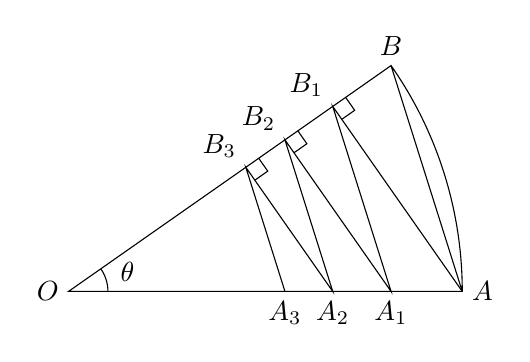
\begin{tikzpicture}[scale = 5]
        \draw (0,0) node [left] {$O$} coordinate (O);
        \draw (1,0) node [right] {$A$} coordinate (A);
        \draw (35:1) node [above] {$B$} coordinate (B);
        \draw (O) -- (A) -- (B) -- cycle (A) arc (0:35:1);
        \draw ($(O)!{cos(35)}!(B)$) node [above left] {$B_1$} coordinate (B1) ($(O)!{cos(35)}!(A)$) node [below] {$A_1$} coordinate (A1);
        \draw ($(O)!{cos(35)}!(B1)$) node [above left] {$B_2$} coordinate (B2) ($(O)!{cos(35)}!(A1)$) node [below] {$A_2$} coordinate (A2);
        \draw ($(O)!{cos(35)}!(B2)$) node [above left] {$B_3$} coordinate (B3) ($(O)!{cos(35)}!(A2)$) node [below] {$A_3$} coordinate (A3);
        \draw (A) -- (B1) -- (A1) -- (B2) -- (A2) -- (B3) -- (A3);
        \pic [draw] {angle = A--O--B}; 
        \draw (0.15,0) node [above] {$\theta$};
        \pic [draw, angle radius = 0.2cm] {right angle = A--B1--B};
        \pic [draw, angle radius = 0.2cm] {right angle = A1--B2--B1};
        \pic [draw, angle radius = 0.2cm] {right angle = A2--B3--B2};      
    \end{tikzpicture}
\end{center}
\item 如图, 在Rt$\triangle ABC$中排列着无限个正方形$S_1,S_2,S_3,S_4,\cdots$, 且已知直角边$BC=a$, 这无限个正方形的面积之和正好是这个直角三角形面积的一半, 求另一直角边$AC$的长.
\begin{center}
    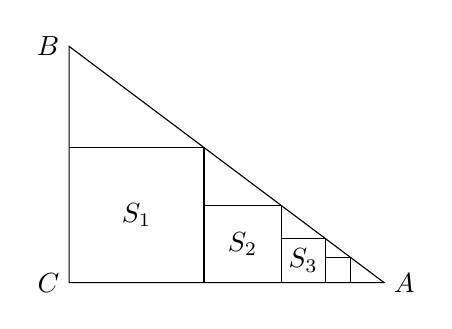
\begin{tikzpicture}
        \draw (0,0) node [left] {$C$} coordinate (C);
        \draw (4,0) node [right] {$A$} coordinate (A);
        \draw (0,3) node [left] {$B$} coordinate (B);
        \draw (A) -- (C) -- (B) -- cycle;
        \draw ({12/7},0) coordinate (X1) -- ({12/7},{12/7}) -- (0,{12/7});
        \draw ({6/7},{6/7}) node {$S_1$};
        \draw (X1) ++ ({12/7*4/7},0) coordinate (X2) --++ (0,{12/7*4/7})  --++ ({-12/7*4/7},0);
        \draw (X1) ++ ({12/7*4/7/2},{12/7*4/7/2}) node {$S_2$};
        \draw (X2) ++ ({12/7*4/7*4/7},0) coordinate (X3) --++ (0,{12/7*4/7*4/7}) --++ ({-12/7*4/7*4/7},0);
        \draw (X2) ++ ({12/7*4/7*4/7/2},{12/7*4/7*4/7/2}) node {$S_3$};
        \draw (X3) ++ ({12/7*4/7*4/7*4/7},0) coordinate (X3) --++ (0,{12/7*4/7*4/7*4/7}) --++ ({-12/7*4/7*4/7*4/7},0);
    \end{tikzpicture}
\end{center}
\item 在半径为$r$的球内作正方体, 然后在正方体内再作内切球, 在内切球内再作内接正方体, 然后再作它的内切球, 如此无限地作下去, 求所有这些球的表面积之和(包括半径为$r$的球).
\item 用数学归纳法证明: $1+2+\cdots +2n=n(2n+1)$($n\in \mathbf{N}^*$).
\item 用数学归纳法证明: $\sqrt {1\times 2}+\sqrt {2\times 3}+\cdots +\sqrt {n(n+1)}>\dfrac{n(n+1)}2$($n\in \mathbf{N}^*$). 
\item 用数学归纳法证明: $1\times n+2(n-1)+\cdots +n\times 1=\dfrac{n(n+1)(n+2)}6$($n\in \mathbf{N}^*$).
\item 记$S_n=1+\dfrac 12+\dfrac 13+\cdots +\dfrac 1n$($n>1$, $n\in \mathbf{N}^*$), 求证: $S_{2^n}>1+\dfrac n2$($n\ge 2$, $n\in \mathbf{N}^*$).\\
解答在这里  (1) 当$n=2$时, $S_{2^2}=1+\dfrac 12+\dfrac 13+\dfrac 14=\dfrac{25}{12}>1+\dfrac 22$, 所以当$n=2$时, 命题成立.\\
(2) 设$n=k$时, 命题成立, 即$S_{2^k}=1+\dfrac 12+\dfrac 13+\cdots +\dfrac 1{2^k}>1+\dfrac k2$,
则$n=k+1$时,
$S_{2^{k+1}}=1+\dfrac 12+\dfrac 13+\cdots +\dfrac 1{2^k}+\dfrac 1{2^k+1}+\dfrac 1{2^k+2}+\cdots +\dfrac 1{2^{k+1}}$
$>1+\dfrac k2+\underbrace{\dfrac 1{2^k+1}+\dfrac 1{2^k+2}+\cdots +\dfrac 1{2^k+2^k}}_{2^k\text{项}}>1+\dfrac k2+\dfrac{2^k}{{2^k}+{2^k}}=1+\dfrac k2+\dfrac 12=1+\dfrac{k+1}2$.\\
故当$n=k+1$时, 命题也成立.
由(1), (2)可知, 对$n\in \mathbf{N}^*$, $n\ge 2$, $S_{2^n}>1+\dfrac n2$.
\item 求证: $a^{n+1}+(a+1)^{2n-1}$($n\in \mathbf{N}^*$)能被$a^2+a+1$整除.\\
解答在这里  (1) 当$n=1$时, $a^{1+1}+(a+1)^{2\times 1-1}=a^2+a+1$, 命题显然成立.\\
(2) 假设当$n=k$时, $a^{k-1}+(a+1)^{2k-1}$能被$a^2+a+1$整除, 则当$n=k+1$时,$a^{k+2}+(a+1)^{2k+1}=a\cdot a^{k+1}+(a+1)^2(a+1)^{2k-1}=a[a^{k+1}+(a+1)^{2k-1}]+(a+1)^2(a+1)^{2k-1}-a(a+1)^{2k-1}=a[a^{k+1}+(a+1)^{2k-1}]+(a^2+a+1)(a+1)^{2k-1}$. 由归纳假设, 以上两项均能被$a^2+a+1$整除, 故$n=k+1$时, 命题也成立.\\
由(1), (2)可知, 对$n\in \mathbf{N}^*$命题成立.
\item 已知数列$\{a_n\}$满足$a_1=a$, $a_{n+1}=\dfrac 1{2-a_n}$.\\
(1) 求$a_2,a_3,a_4$;\\
(2) 推测通项$a_n$的表达式, 并用数学归纳法加以证明.\\
解答在这里  (1) 由$a_{n+1}=\dfrac 1{2-a_n}$, 可得$a_2=\dfrac 1{2-a}$, $a_3=\dfrac 1{2-\dfrac 1{2-a}}=\dfrac{2-a}{3-2a}$, $a_4=\dfrac 1{2-\dfrac{2-a}{3-2a}}=\dfrac{3-2a}{4-3a}$.\\
(2) 推测$a_n=\dfrac{(n-1)-(n-2)a}{n-(n-1)a}$, 证明如下:
\textcircled{1} 当$n=1$时, 左边$=a_1=a$, 右边$=\dfrac{(1-1)-(1-2)a}{1-(1-1)a}=a$, 结论成立.
\textcircled{2} 设$n=k$时, 有$a_k=\dfrac{(k-1)-(k-2)a}{k-(k-1)a}$,
则当$n=k+1$时,
$a_{k+1}=\dfrac 1{2-a_k}=\dfrac 1{2-\dfrac{(k-1)-(k-2)a}{k-(k-1)a}}=\dfrac{k-(k-1)a}{2[k-(k-1)a]-[(k-1)-(k-2)a]}=\dfrac{k-(k-1)a}{(k+1)-ka}$.
故当$n=k+1$时, 结论成立.\\
由\textcircled{1} , \textcircled{2} 可知, 对$n\in \mathbf{N}^*$, 都有$a_n=\dfrac{(n-1)-(n-2)a}{n-(n-1)a}$.
\item 平面内有$n$个圆, 其中每两个圆都交于两点, 且无任何三个圆交于一点, 求证: 这$n$个圆将平面分成$n^2-n+2$个部分.\\
解答在这里 设$n=k$时, $k$个圆将平面分成$k^2-k+2$个部分(如图), 则当$n=k+1$时, 第$k+1$个圆$C_{k+1}$交前面$k$个圆于$2k$个点, 这$2k$个点将圆$C_{k+1}$分成$2k$段, 每段将各自所在区域一分为二, 因此增加了$2k$个区域, 于是这$k+1$个圆将平面分成$k^2-k+2+2k$个部分, 即$(k+1)^2-(k+1)+2$个部分.
\begin{center}
    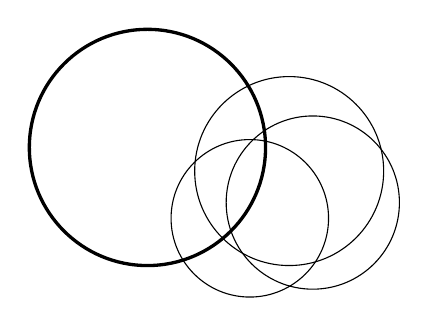
\begin{tikzpicture}
        \draw (0,0) circle (1);
        \draw (0.5,0.6) circle (1.2);
        \draw (0.8,0.2) circle (1.1);
        \draw [very thick] (-1.3,0.9) circle (1.5);
    \end{tikzpicture}
\end{center}
\item 利用数学归纳法证明``$1+a+a^2+\cdots +a^{n+1}=\dfrac{1-{a^{n+2}}}{1-a}$($a\ne 1$, $n\in \mathbf{N}^*$)''时, 在验证$n=1$成立时, 左边应该是\bracket{20}.
\fourch{$1$}{$1+a$}{$1+a+a^2$}{$1+a+a^2+a^3$}
\item 欲用数学归纳法证明``对于足够大的自然数$n$, 总有$2^n>n^3$'', 则验证不等式成立所取的第一个$n$值, 最小应当是\bracket{20}.
\twoch{$1$}{大于$1$且小于$6$的某个自然数}{$10$}{大于$5$且小于$10$的某个自然数}
\item 利用数学归纳法证明``对任意偶数$n$, $a^n-b^n$能被$a+b$整除''时, 其第二步论证, 应该是\bracket{20}.
\onech{假设$n=k$时命题成立, 再证$n=k+1$时命题也成立}{假设$n=2k$时命题成立, 再证$n=2k+1$时命题也成立}{假设$n=k$时命题成立, 再证$n=k+2$时命题也成立}{假设$n=2k$时命题成立, 再证$n=2(k+1)$时命题也成立}
\item 利用数学归纳法证明``$(n+1)(n+2)(n+3)\cdots (n+n)=2^n\times 1\times 3\times \cdots \times (2n-1)$($n\in \mathbf{N}^*$)''时, 从``$n=k$''变到``$n=k+1$''时, 左边应增添的因式是\bracket{20}.
\fourch{$2k+1$}{$\dfrac{2k+1}{k+1}$}{$\dfrac{(2k+1)(2k+2)}{k+1}$}{$\dfrac{2k+3}{k+1}$}
\item 利用数学归纳法证明``$\dfrac 1{n+1}+\dfrac 1{n+2}+\cdots +\dfrac 1{2n}>\dfrac{13}{24}$($n\ge 2$, $n\in \mathbf{N}^*$)''的过程中, 由``$n=k$''变到``$n=k+1$''时, 不等式左边的变化是\bracket{20}.
\twoch{增加$\dfrac 1{2(k+1)}$}{增加$\dfrac 1{2k+1}$和$\dfrac 1{2k+2}$}{增加$\dfrac 1{2k+2}$并减少$\dfrac 1{k+1}$}{增加$\dfrac 1{2k+1}$和$\dfrac 1{2k+2}$, 并减少$\dfrac 1{k+1}$.}
\item 利用数学归纳法证明不等式``$\sqrt {n^2+n}<n+1$''时, 由``假设$n=k$时命题成立''到``当$n=k+1$时'', 正确的步骤是\bracket{20}.
\onech{$\sqrt {(k+1)^2+(k+1)}=\sqrt {k^2+3k+2}<\sqrt {k^2+4k+4}=k+2$}{$\sqrt {(k+1)^2+(k+1)}=\sqrt {k^2+3k+2}=\sqrt {(k+2)^2-(k+2)}<k+2$}{$\sqrt {(k+1)^2+(k+1)}=\sqrt {k^2+3k+2}<\sqrt {(k+2)^2}=k+2$}{$\sqrt {(k+1)^2+(k+1)}=\sqrt {k^2+3k+2}=\sqrt {(k^2+k)+2k+2}<\sqrt {(k+1)^2+2k+2}=\sqrt {(k+2)^2-1}<\sqrt {(k+2)^2}=k+2$}
\item 利用数学归纳证明不等式``$1+\dfrac 12+\dfrac 13+\cdots +\dfrac 1{2^n-1}<n$($n\ge 2$, $n\in \mathbf{N}^*$)''的过程中, 由``$n=k$''变到``$n=k+1$''时, 左边增加了\bracket{20}.
\fourch{$1$项}{$k$项}{$2^{k-1}$项}{$2^k$项}
\item 利用数学归纳法证明: $1+2+3+\cdots +2n=n(2n+1)$($n\in \mathbf{N}^*$).
\item 利用数学归纳法证明: $1^2-2^2+3^2-4^2+\cdots +(-1)^{n-1}n^2=(-1)^{n-1}\cdot \dfrac{n(n+1)}2$($n\in \mathbf{N}^*$).
\item 利用数学归纳法证明: $1-\dfrac 12+\dfrac 13-\dfrac 14+\cdots +\dfrac 1{2n-1}-\dfrac 1{2n}=\dfrac 1{n+1}+\dfrac 1{n+2}+\cdots +\dfrac 1{2n}$($n\in \mathbf{N}^*$).
\item 利用数学归纳法证明: $1^3+2^3+3^3+\cdots +n^3=\dfrac 14[n(n+1)]^2$($n\in \mathbf{N}^*$).
\item 利用数学归纳法证明: $(1\times 2^2-2\times 3^2)+(3\times 4^2-4\times 5^2)+\cdots +[(2n-1)(2n)^2-2n(2n+1)^2] \\ =-n(n+1)(4n+3)$($n\in \mathbf{N}^*$).
\item 对于$n\in \mathbf{N}^*$, 求证: $\dfrac 12\tan \dfrac x2+\dfrac 1{2^2}\tan \dfrac x{2^2}+\cdots +\dfrac 1{2^n}\tan \dfrac x{2^n}=\dfrac 1{2^n}\cot \dfrac x{2^n}-\cot x$($x\ne k\pi$, $n\in \mathbf{Z}$).
\item 对于$n\in \mathbf{N}^*$, 求证: $\dfrac 1{\cos \alpha \cos (\alpha +\beta)}+\dfrac 1{\cos (\alpha +\beta)\cos (\alpha +2\beta)}+\cdots +\dfrac 1{\cos [\alpha +(n-1)\beta]\cos (\alpha +n\beta)} \\ =\dfrac{\sin n\beta }{\sin \beta \cos \alpha (\alpha +n\beta)}$.
\item 对于$n\in \mathbf{N}^*$, 求证: $(2\cos \theta -1)(2\cos 2\theta -1)(2\cos 2^2\theta -1)\cdots (2\cos 2^{n-1}\theta -1)=\dfrac{2\cos {2^n}\theta +1}{2\cos \theta +1}$(其中$\theta \ne 2k\pi \pm \dfrac{2\pi }3$, $k\in \mathbf{Z}$).
\item 对于$n\in \mathbf{N}^*$, 求证: $\dfrac 1{\sin 2x}+\dfrac 1{\sin 4x}+\cdots +\dfrac 1{\sin 2^nx}=\cot x-\cot 2^nx$($x\ne \dfrac{m\pi }{2^p}$, $m\in \mathbf{Z}$, $p\in \mathbf{N}^*$).
\item 在数列$\{a_n\}$中, 已知$a_1=1$, $a_{n+1}=6(1+2+\cdots +n)+1$($n\in \mathbf{N}^*$), 求证: $a_1+a_2+\cdots +a_n=n^3$.
\item 设$x_1,x_2$是关于$x$的方程$2x^2+2nx-n=0$($n\in \mathbf{N}^*$)的两个根, 数列$\{a_n\}$的通项$a_n=x_1^2+x_2^2$, 试用数学归纳法证明: 对任何自然数$n$, 都有$\dfrac 1{1+a_1}+\dfrac 1{2+a_2}+\dfrac 1{3+a_3}+\cdots +\dfrac 1{n+a_n}=\dfrac{n(3n+5)}{4(n+1)(n+2)}$.
\item 利用数学归纳法证明: $\dfrac 1{n+1}+\dfrac 1{n+2}+\dfrac 1{n+3}+\cdots +\dfrac 1{2n}>\dfrac{13}{24}$($n\ge 2$, $n\in \mathbf{N}^*$).
\item 利用数学归纳法证明: $\dfrac 1{n+1}+\dfrac 1{n+2}+\cdots +\dfrac 1{3n+2}>1$($n\in \mathbf{N}^*$).
\item 利用数学归纳法证明: $\dfrac 1n+\dfrac 1{n+1}+\dfrac 1{n+2}+\cdots +\dfrac 1{n^2}>1$($n\ge 2$, $n\in \mathbf{N}^*$).
\item 利用数学归纳法证明: $1+\dfrac 12+\dfrac 13+\cdots +\dfrac 1{2^n-1}<n$($n\ge 2$, $n\in \mathbf{N}^*$).
\item 已知$n\in \mathbf{N}^*$, 求证: $|\sin \theta|\le n|\sin \theta|$.
\item 已知$n\in \mathbf{N}^*$, 求证: $\cot \dfrac{\theta }{2^n}-\cot \theta \ge n$($0<\theta <\pi$).
\item 利用数学归纳法证明:$(1+\dfrac 1n)^n<n$($n\ge 3$, $n\in \mathbf{N}^*$).
\item 利用数学归纳法证明:$\dfrac{{2^n}-1}{{2^n}+1}>\dfrac n{n+1}$($n\ge 3$, $n\in \mathbf{N}^*$).
\item 利用数学归纳法证明:$\dfrac{2^n+4^n}2\ge 3^n$($n\in \mathbf{N}^*$).
\item 利用数学归纳法证明:$\dfrac{a^n+b^n}2\ge (\dfrac{a+b}2)^n$($a,b\in \mathbf{R}^+$, $n\in \mathbf{N}^*$).
\item 利用数学归纳法证明:$(2n+1)(1-x)x^n<1-x^{2n+1}$($0<x<1$, $n\in \mathbf{N}^*$).
\item 已知数列$\{a_n\}$满足$a_1=2$, $a_{n+1}=\dfrac{a_n}2+\dfrac 1{a_n}$, 求证: $\sqrt 2<a_n<\sqrt 2+\dfrac 1n$.
\item 求证: $49^n+16n-1$能被$64$整除($n\in \mathbf{N}^*$).
\item 求证: $6^{2n}+3^{n+2}+3^n$是$11$的倍数($n\in \mathbf{N}^*$).
\item 求证: $7^n+1$能被$8$整除, 其中$n$为正奇数.
\item 求证: $(3n+1)\times 7^n-1$是$9$的倍数($n\in \mathbf{N}^*$).
\item 求证: $1+2+2^2+2^3+\cdots +2^{5n-1}$能被$31$整除($n\in \mathbf{N}^*$).
\item 求证: $(x+3)^n-1$能被$x+2$整除($n\in \mathbf{N}^*$).
\item 求证: $x^n-na^{n-1}x+(n-1)a^n$能被$(x-a)^2$整除($n\ge 2$, $n\in \mathbf{N}^*$).
\item 当$n\in \mathbf{N}^*$时, 试用数学归纳法证明$f(n)=n^3+\dfrac 32n^2+\dfrac 12n-1$一定是整数.
\item 已知数列$\{a_n\}$满足$a_1=1$, $a_{n+1}=\dfrac{a_n}{1+{a_n}}$.\\
(1) 计算$a_2,a_3,a_4$;\\
(2) 猜测$a_n$的表达式, 并用数学归纳法加以证明.
\item 已知数列$\{a_n\}$的通项公式是$a_n=\dfrac 1{(n+1)^2}$($n\in \mathbf{N}^*$), 记$b_n=(1-a_1)(1-a_2)\cdots (1-a_n)$.\\
(1) 写出数列$\{b_n\}$的前三项;\\
(2) 猜想数列$\{b_n\}$的通项公式, 并用数学归纳法加以证明;\\
(3) 令$p_n=b_n-b_{n+1}$, 求$\displaystyle \lim_{n\to \infty} (p_1+p_2+\cdots +p_n)$的值.
\item 已知$a>0$, $b>0$, 数列$\{a_n\}$满足$a_1=\dfrac 12(a+\dfrac ba),a_2=\dfrac 12(a_1+\dfrac b{a_1}),a_3=\dfrac 12(a_2+\dfrac b{a_2}),\cdots,a_n=\dfrac 12(a_{n-1}+\dfrac b{a_{n-1}})$.\\
(1) 求证: $\dfrac{{a_n}-\sqrt b}{{a_n}+\sqrt b}=(\dfrac{a-\sqrt b}{a+\sqrt b})^{2n}$;\\
(2) 求$\displaystyle \lim_{n\to \infty} a_n$.
\item 已知正数数列$\{a_n\}$满足$2\sqrt {S_n}=a_n+1$($n\in \mathbf{N}^*$).\\
(1) 求$a_1,a_2,a_3$;\\
(2) 猜测$a_n$的表达式, 并证明你的结论.
\item 已知正数数列$\{a_n\}$的前$n$项和$S_n$满足$S_n=\dfrac 12(a_n+\dfrac 1{a_n})$, 求$a_n$.
\item 已知正数数列$\{a_n\}$的前$n$项和$S_n=\dfrac 12(a_n+\dfrac 1{a_n})$.\\
(1) 求$S_1,S_2,S_3$;\\
(2) 写出$S_n$的表达式, 并证明你的结论;\\
(3) 求$\displaystyle \lim_{n\to \infty} a_n$.
\item 已知正数数列$\{a_n\}$的前$n$项和为$S_n$, 且对任何自然数$n$, $a_n$与$2$的等差中项等于$S_n$与$2$的正的等比中项.\\
(1) 写出数列$\{a_n\}$的前三项;\\
(2)求数列$\{a_n\}$的通项公式(写出证明过程).
\item 已知$n\in \mathbf{N}^*$, 比较$\dfrac 12\times \dfrac 34\times \dfrac 56\times \cdots \times \dfrac{2n-1}{2n}$与$\dfrac 1{2\sqrt n}$的大小.
\item 已知$n\in \mathbf{N}^*$, 比较$(n+1)^2$与$3^n$的大小.
\item 已知数列$\{a_n\}$满足$a_1=2$, $a_{n+1}=\dfrac{{a_n}^2+3}{2{a_n}}$, 数列$\{b_n\}$满足$b_n=3-a_n^2$.求证:\\
(1) $b_n<0$;\\
(2) $|\dfrac{{b_{n+1}}}{b_n}|<\dfrac 12$;\\
(3) $|b_n|<(\dfrac 12)^{n-1}$($n\ge 2$).
\item 已知数列$\{a_n\}$满足条件$a_1=1$, $a_2=r$($r>0$), 且$\{a_na_{n+1}\}$是公比为$q$($q>0$)的等比数列, 记$b_n=a_{2n-1}+a_{2n}$($n\in \mathbf{N}^*$).\\
(1) 求出使不等式$a_na_{n+1}+a_{n+1}a_{n+2}>a_{n+2}a_{n+3}$成立的$q$的取值范围;\\
(2) 求$b_n$和$\displaystyle \lim_{n\to \infty} \dfrac 1{S_n}$, 其中$S_n=b_1+b_2+\cdots +b_n$.
\item 平面上有$n$条直线, 其中任何两条都不平行, 任何三条不共点, 求证这$n$条直线:\\
(1) 被分割成$n^2$段.\\
(2) 把平面分成$\dfrac 12(n^2+n+2)$个部分.
\item 已知一个圆内有$n$条弦, 这$n$条弦中每两条都相交于圆内的一点, 且任何三条不共点, 求证: 这$n$条弦将圆面分割成$f(n)=\dfrac 12n^2+\dfrac 12n+1$个区域.
\item 数列$2, 0, 4, 0, 6, 0, \cdots$的一个通项公式是\bracket{20}.
\twoch{$a_n=\dfrac{n[1+(-1)^n]}2$}{$a_n=\dfrac{(n+1)[1+(-1)^n]}2$}{$a_n=\dfrac{n[1+(-1)^{n+1}]}2$}{$a_n=\dfrac{(n+1)[1+(-1)^{n+1}]}2$}
\item 在数列$\{a_n\}$中, 已知$a_1=2$, $a_{n+1}=a_n+2n$, 则$a_{100}$等于\bracket{20}.
\fourch{$9900$}{$9902$}{$9904$}{$10100$}
\item 已知数列$\{a_n\}$满足$a_1=4$, $a_2=2$, $a_3=1$, 又数列$\{a_{n+1}-a_n\}$成等差数列, 则$a_n$等于\bracket{20}.
\twoch{$n-3$}{$\dfrac 12(n^3-8n^2+13n+2)$}{$\dfrac 12(2n^3-17n^2+33n-10)$}{$\dfrac 12(n^2-7n+14)$}
\item 求数列$23, 2323, 232323, \cdots$的通项公式$a_n$.
\item 求数列$\sqrt {11-2},\sqrt {1111-22},\cdots,\sqrt {\underbrace{11\cdots 11}_{2n}-\underbrace{22\cdots 22}_{n}}, \cdots$的前$n$项和$S_n$.
\item 求证: $12, 1122, 111222, \cdots$的每一项都是两个相邻整数之积.
\item 已知数列$\{a_n\}$满足$a_{n+1}=2a_n+3$, 且$a_1\ne -3$.\\
(1) 求证: 数列$\{a_n+3\}$成等比数列;\\
(2) 若$a_1=5$, 求$a_n$.
\item 已知数列$\{a_n\}$满足$a_1=1$, $a_{n+1}=S_n+(n+1)$.\\
(1) 用$a_n$表示$a_{n+1}$;\\
(2) 求证: 数列$\{a_n+1\}$成等比数列;\\
(3) 求$a_n$和$S_n$.
\item 已知数列$\{a_n\}$满足$a_1=\dfrac 56$, 且关于$x$的二次方程$a_{k-1}x^2-a_kx+1=0$的两根$\alpha ,\beta$满足$3\alpha -\alpha \beta +3\beta =1$($k\ge 2$, $k\in \mathbf{N}^*$), 求证: 数列$\{a_n-\dfrac 12\}$是等比数列, 并求出通项$a_n$.
\item 求和: $\dfrac 12+(\dfrac 13+\dfrac 23)+(\dfrac 14+\dfrac 24+\dfrac 34)+\cdots +(\dfrac 1{100}+\dfrac 2{100}+\dfrac 3{100}+\cdots +\dfrac{99}{100})$.
\item 将自然数按下表排列:
\[\begin{array}{cccccc}
1&2&5&10&17&\cdots \\
4&3&6&11&18&\cdots \\
9&8&7&12&19&\cdots \\
16&15&14&13&20&\cdots \\
25&24&23&22&21&\cdots \\
\cdots&\cdots&\cdots&\cdots&\cdots&\cdots	
\end{array}\]		
(1) 第$1$列中第$m$个数是多少? 第$1$行中第$n$个数是多少?\\
(2) 若$m\ge n$, 则第$m$行(自上而下)、第$n$列(自左而右)的数是多少? 若$m<n$呢?\\
(3) $99$在上起第几行、左起第几列?
\item 已知数列$1,\dfrac 12,\dfrac 21,\dfrac 13,\dfrac 22,\dfrac 31,\dfrac 14,\dfrac 23,\dfrac 32,\dfrac 41,\cdots$.\\
(1) 试按照规律, 将此数列分组;\\
(2) 分数$\dfrac nm$($m,n\in \mathbf{N}^*$, $m,n$互质)属于第几组第几项?\\
(3) $\dfrac{17}{30}$是此数列的第几项?\\
(4) 数列的第$50$项是多少?
\item 已知数列$\{a_n\}$的前$n$项之和$S_n$与$a_n$之间满足$2S_n^2=2a_nS_n-a_n$($n\ge 2$), 且$a_1=2$.\\
(1) 求证: 数列$\{\dfrac 1{S_n}\}$是以$2$为公差的等差数列;\\
(2) 求$S_n$和$a_n$.
\item 在数列$\{a_n\}$中, 已知$a_1=1$, $a_n=\dfrac{2S_n^2}{2{S_n}-1}$($n\ge 2$).\\
(1) 求证: $\{\dfrac 1{S_n}\}$成等差数列;\\
(2) 求通项$a_n$的表达式.
\item 已知数列$\{a_n\}$, $\{b_n\}$的通项公式分别是$a_n=2^n$, $b_n=3n+2$, 将它们的公共项由小到大排成数列$\{c_n\}$, 求数列$\{c_n\}$的通项公式.
\item 已知数列$\{a_n\}$满足$a_{n+1}=3^na_n$, 且$a_1=1$, 求$a_n$.
\item 已知数列$\{a_n\}$满足$a_1=\dfrac 12$, $S_n=n^2a_n$($S_n$是前$n$项之和), 求$a_n$.
\item 已知数列$\{a_n\}$满足$a_1=1$, $a_n+a_{n+1}=-2n$.\\
(1) 求证: 数列$\{a_{2n}\}$与$\{a_{2n-1}\}$均是以$-2$为公差的等差数列;\\
(2) 试用$n$表示和式$M=a_1a_2-a_2a_3+\cdots +(-1)^{k+1}\cdot a_ka_{k+1}+\cdots +a_{2n-1}a_{2n}-a_{2n}a_{2n+1}$.
\item 是否可找到$2n+1$个连续自然数($n\in \mathbf{N}^*$), 使得前$n+1$个数的平方和等于末$n$个数的平方和? 此时中间数可取什么?
\item 是否存在常数$k$和等差数列$\{a_n\}$, 使得$ka_n^2-1=S_{2n}-S_{n+1}$对任何$n\in \mathbf{N}^*$都成立($S_n$为等差数列$\{a_n\}$前$n$项之和)?
\item 在直角$\triangle ABC$中, 已知$\angle C=90^\circ$, $AC=b$, $AB=c$, 将斜边$AB$分成$n+1$等份, 记分点为$P_1,P_2,\cdots,P_n$, 连接$CP_1,CP_2,\cdots,CP_n$, 求$\displaystyle \lim_{n\to \infty} \dfrac 1n[(CP_1)^2+(CP_2)^2+\cdots +(CP_n)^2]$.
\item 已知各项为正数的数列$\{a_n\}$满足$a_n^2\le a_n-a_{n+1}$, 求证$a_n<\dfrac 1n$.
\item 已知各项为正数的数列$\{a_n\}$满足$a_1+a_2+\cdots +a_n=1$, 求证: $a_1^2+a_2^2+\cdots +a_n^2\ge \dfrac 1n$($n\ge 2$).
\item 已知$\dfrac 12\le a_k\le 1$($k\in \mathbf{N}^*$), 求证: $a_1a_2\cdots a_n+(1-a_1)(1-a_2)\cdots (1-a_n)\ge \dfrac 1{2^{n-1}}$.
\item 已知$\{a_n\}$, $\{b_n\}$是满足$(1+\sqrt 2)^n=a_n+b_n\sqrt 2$的两个无穷数列.\\
(1) 推测用$a_n$, $b_n$表示$(1-\sqrt 2)^n$的表达方式, 并加以证明;\\
(2) 求: $\displaystyle \lim_{n\to \infty} \dfrac{b_n}{a_n}$.


\end{enumerate}
\end{document}